\section{Casi d'uso}
\subsection{Introduzione}
In questa sezione del documento vengono analizzati nel dettaglio i casi d'uso individuati per il sistema.
nel corso dell'analisi del \href{https://7last.github.io/docs/rtb/documentazione-interna/glossario\#capitolato}{capitolato\textsubscript{G}} e dei colloqui con la \href{https://7last.github.io/docs/rtb/documentazione-interna/glossario\#proponente}{proponente\textsubscript{G}}.

\subsection{Struttura dei casi d'uso}
In tutto il documento ci si riferirà ai casi d'uso utilizzando la sigla \texttt{UC} seguita dal rispettivo codice nella forma
\begin{center}
	\textbf{UC-[identificativo\_caso\_principale].[identificativo\_sotto\_caso]}
\end{center}

il quale permette di utilizzarlo come riferimento in questo e altri documenti.\\
Per ciascun caso d'uso vengono definiti i seguenti elementi:
\begin{itemize}
	\item \textbf{Attore principale}: l'attore primariamente coinvolto nel caso d'uso;
	\item \textbf{Precondizioni}: le condizioni che devono essere verificate affinché il caso d'uso possa essere
	      eseguito;
	\item \textbf{Postcondizioni}: le condizioni che devono essere verificate al termine dell'esecuzione del caso
	\item \textbf{Scenario principale}: la sequenza di passi che descrive il comportamento del sistema durante
	      l'esecuzione del caso d'uso;
	\item \href{https://7last.github.io/docs/rtb/documentazione-interna/glossario\#user-story}{\textbf{User story}\textsubscript{G}}: una descrizione testuale del caso d'uso.
\end{itemize}


\subsection{Attori}
I seguenti attori sono coinvolti nei casi d'uso:
\begin{itemize}
	\item Impiegati presso \textbf{autorità locali}: essi possono accedere al sistema per visualizzare i dati
	      monitoraggio della \href{https://7last.github.io/docs/rtb/documentazione-interna/glossario\#smart-city}{\textit{Smart City}\textsubscript{G}}.
	\item \textbf{Sensori}: sorgente di dati con un determinato dominio di interesse che effettua misurazioni
	      e trasmette i dati al sistema.
\end{itemize}

\subsection{Elenco dei casi d'uso}
\subsubsection{UC-1: Visualizzazione dashboard generale}
\begin{itemize}
	\item \textbf{Attore principale}: Autorità locale;
	\item \textbf{Precondizioni}: L'autorità locale ha effettuato l'accesso al sistema ed esso è in funzione;
	\item \textbf{Postcondizioni}: L'autorità locale visualizza la \href{https://7last.github.io/docs/rtb/documentazione-interna/glossario\#dashboard}{dashboard\textsubscript{G}} generale con i dati relativi ai sensori
	      presenti nella città;
	\item \textbf{Scenario principale}:
	      \begin{enumerate}
		      \item L'autorità locale accede alla piattaforma;
		      \item Il sistema carica i dati relativi ai sensori interrogando il database.
	      \end{enumerate}
	\item \href{https://7last.github.io/docs/rtb/documentazione-interna/glossario\#user-story}{\textbf{User story}\textsubscript{G}}: Come autorità locale desidero poter visualizzare una \href{https://7last.github.io/docs/rtb/documentazione-interna/glossario\#dashboard}{dashboard\textsubscript{G}} generale con i dati relativi ai sensori presenti,
	      la quale mi consente di monitorare quanti, quali sensori sono presenti e la loro posizione.
\end{itemize}
\begin{center}
	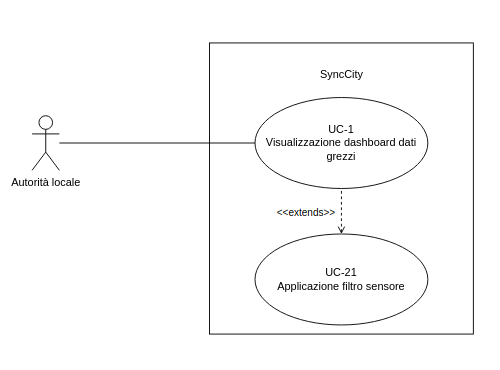
\includegraphics[width=0.6\textwidth]{analisi_dei_requisiti/UC-1.png}
	\captionof{figure}{UC-1: Visualizzazione \href{https://7last.github.io/docs/rtb/documentazione-interna/glossario\#dashboard}{dashboard\textsubscript{G}} generale}
\end{center}

\subsubsubsection{UC-1.1: Visualizzazione panel con tabella sensori}
\begin{itemize}
	\item \textbf{Attore principale}: Autorità locale;
	\item \textbf{Precondizioni}:
	      \begin{enumerate}
		      \item L'autorità locale ha effettuato l'accesso al sistema ed esso è in funzione;
	      \end{enumerate}
	\item \textbf{Postcondizioni}:
	      L'autorità locale visualizza il \textit{panel} contenente una tabella di tutti i sensori collegati al sistema;

	\item \textbf{Scenario principale}:
	      \begin{enumerate}
		      \item L'autorità locale accede alla piattaforma;
		      \item Il sistema carica i dati relativi ai sensori interrogando il database;
		      \item L'autorità locale seleziona la visualizzazione della \href{https://7last.github.io/docs/rtb/documentazione-interna/glossario\#dashboard}{dashboard\textsubscript{G}} generale.
	      \end{enumerate}
	\item \href{https://7last.github.io/docs/rtb/documentazione-interna/glossario\#user-story}{\textbf{User story}\textsubscript{G}}: Come autorità locale desidero poter visualizzare un panel contenente una tabella di tutti i sensori collegati al sistema.
	      I dati che dovranno essere presenti nella tabella sono: identificativo del \href{https://7last.github.io/docs/rtb/documentazione-interna/glossario\#sensore}{sensore\textsubscript{G}}, posizione e tipo di \href{https://7last.github.io/docs/rtb/documentazione-interna/glossario\#sensore}{sensore\textsubscript{G}}.
	      I dati presenti nella tabella mi consentiranno di avere una visione d'insieme dei sensori presenti.

\end{itemize}
\begin{center}
	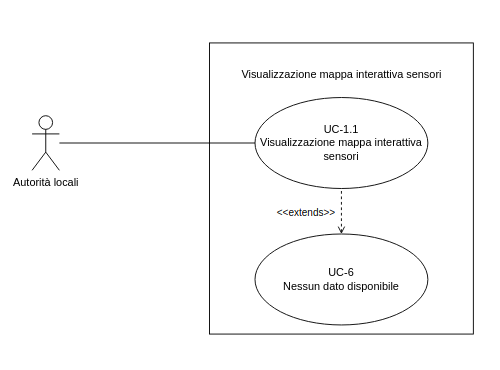
\includegraphics[width=0.6\textwidth]{analisi_dei_requisiti/UC-1.1.png}
	\captionof{figure}{UC-1.1: Visualizzazione panel con tabella sensori}
\end{center}

\subsubsubsection{UC-1.2: Visualizzazione mappa interattiva sensori}
\begin{itemize}
	\item \textbf{Attore principale}: Autorità locale;
	\item \textbf{Precondizioni}: L'autorità locale ha effettuato l'accesso al sistema ed esso è in funzione;
	\item \textbf{Postcondizioni}: L'autorità locale visualizza un \textit{panel} contenente una mappa interattiva
	      popolata con dei marker rappresentanti la posizione dei sensori;
	\item \textbf{Scenario principale}:
	      \begin{enumerate}
		      \item L'autorità locale accede alla piattaforma;
		      \item Il sistema carica i dati trasmessi dai sensori interrogando il database;
		      \item L'autorità locale seleziona la visualizzazione della \href{https://7last.github.io/docs/rtb/documentazione-interna/glossario\#dashboard}{dashboard\textsubscript{G}} generale.
	      \end{enumerate}
	\item \href{https://7last.github.io/docs/rtb/documentazione-interna/glossario\#user-story}{\textbf{User story}\textsubscript{G}}: Come autorità locale desidero poter visualizzare una mappa interattiva popolata con dei marker rappresentanti
	      la posizione dei sensori e contenenti il loro identificativo. Essa mi consentirà di visualizzare la distribuzione dei sensori nel territorio
	      ed eventualmente interventire nel caso in cui siano presenti zone non coperte.
\end{itemize}
\begin{center}
	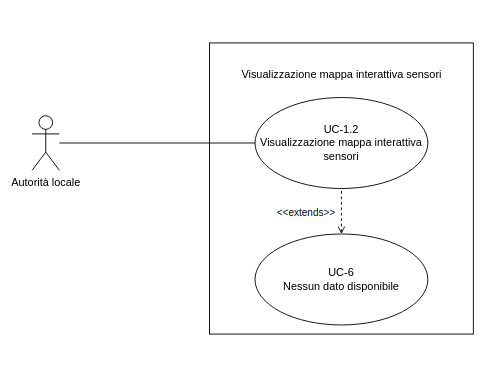
\includegraphics[width=0.6\textwidth]{analisi_dei_requisiti/UC-1.2.png}
	\captionof{figure}{UC-1.2: Visualizzazione mappa interattiva sensori}
\end{center}

\subsubsubsection{UC-1.3: Visualizzazione \textit{panel} numero sensori}
\begin{itemize}
	\item \textbf{Attore principale}: Autorità locale;
	\item \textbf{Precondizioni}: L'autorità locale ha effettuato l'accesso al sistema ed esso è in funzione;
	\item \textbf{Postcondizioni}: L'autorità locale visualizza un \textit{panel} contenente il conteggio totale di sensori presenti nel sistema;
	\item \textbf{Scenario principale}:
	      \begin{enumerate}
		      \item L'autorità locale accede alla piattaforma;
		      \item Il sistema carica i dati trasmessi dai sensori interrogando il database;
		      \item L'autorità locale seleziona la visualizzazione della \href{https://7last.github.io/docs/rtb/documentazione-interna/glossario\#dashboard}{dashboard\textsubscript{G}} generale.
	      \end{enumerate}
	\item \href{https://7last.github.io/docs/rtb/documentazione-interna/glossario\#user-story}{\textbf{User story}\textsubscript{G}}:
	      Come autorità locale desidero poter visualizzare il conteggio totale di sensori presenti nel sistema, in modo da poter decidere eventualmente di aggiungerne altri.
\end{itemize}
\begin{center}
	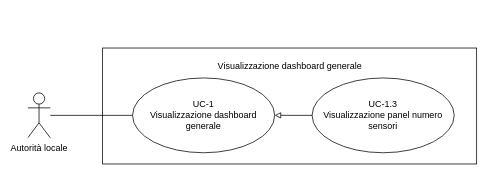
\includegraphics[width=0.6\textwidth]{analisi_dei_requisiti/UC-1.3.png}
	\captionof{figure}{UC-1.3: Visualizzazione \textit{panel} numero sensori}
\end{center}

\subsubsubsection{UC-1.4: Visualizzazione tabella sensori non trasmettenti}
\begin{itemize}
	\item \textbf{Attore principale}: Autorità locale;
	\item \textbf{Precondizioni}: L'autorità locale ha effettuato l'accesso al sistema ed esso è in funzione;
	\item \textbf{Postcondizioni}: L'autorità locale visualizza una tabella contenente i sensori che non trasmettono da più di un giorno;
	\item \textbf{Scenario principale}:
	      \begin{enumerate}
		      \item L'autorità locale accede alla piattaforma;
		      \item Il sistema carica i dati trasmessi dai sensori interrogando il database;
		      \item L'autorità locale seleziona la visualizzazione della \href{https://7last.github.io/docs/rtb/documentazione-interna/glossario\#dashboard}{dashboard\textsubscript{G}} generale.
	      \end{enumerate}
	\item \href{https://7last.github.io/docs/rtb/documentazione-interna/glossario\#user-story}{\textbf{User story}\textsubscript{G}}:
	      Come autorità locale desidero poter visualizzare una tabella contenente i sensori che non trasmettono da più di un giorno, in modo da poter intervenire e ripristinare il corretto funzionamento.
\end{itemize}
\begin{center}
	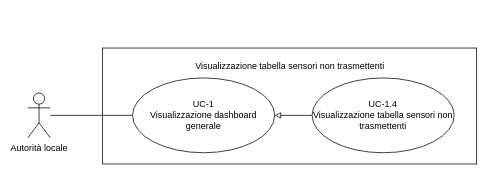
\includegraphics[width=0.6\textwidth]{analisi_dei_requisiti/UC-1.4.png}
	\captionof{figure}{UC-1.4: Visualizzazione tabella sensori che non trasmettono da più di 1 giorno}
\end{center}

\subsubsection{UC-2: Visualizzazione dashboard temperatura}
\begin{itemize}
	\item \textbf{Attore principale}: Autorità locale;
	\item \textbf{Precondizioni}: L'autorità locale ha effettuato l'accesso al sistema ed esso è in funzione;
	\item \textbf{Postcondizioni}: L'autorità locale visualizza la \href{https://7last.github.io/docs/rtb/documentazione-interna/glossario\#dashboard}{dashboard\textsubscript{G}} relativa
	      ai sensori di temperatura presenti nella città;
	\item \textbf{Scenario principale}:
	      \begin{enumerate}
		      \item L'autorità locale accede alla piattaforma;
		      \item Il sistema carica i dati trasmessi dai sensori interrogando il database;
		      \item L'autorità locale seleziona la visualizzazione della \href{https://7last.github.io/docs/rtb/documentazione-interna/glossario\#dashboard}{dashboard\textsubscript{G}} relativa ai sensori di temperatura.
	      \end{enumerate}
	\item \href{https://7last.github.io/docs/rtb/documentazione-interna/glossario\#user-story}{\textbf{User story}\textsubscript{G}}:
	      Come autorità locale desidero poter visualizzare una \href{https://7last.github.io/docs/rtb/documentazione-interna/glossario\#dashboard}{dashboard\textsubscript{G}} relativa ai sensori di temperatura presenti nella città, la quale
	      dovrà contenere informazioni utili per monitorare l'andamento della temperatura sulla base di dati storici e in tempo reale, mostrando
	      anche statistiche quali la temperatura media, massima e minima in un determinato periodo di tempo.
\end{itemize}
\begin{center}
	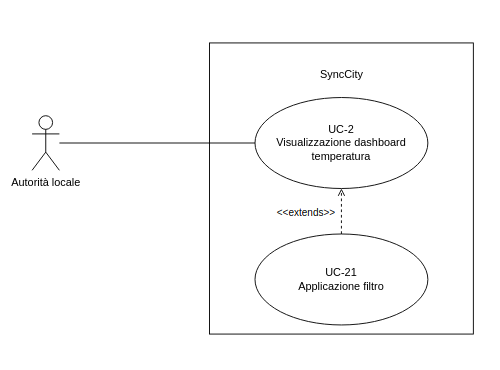
\includegraphics[width=0.6\textwidth]{analisi_dei_requisiti/UC-2.png}
	\captionof{figure}{UC-2: Visualizzazione \href{https://7last.github.io/docs/rtb/documentazione-interna/glossario\#dashboard}{dashboard\textsubscript{G}} temperatura}
\end{center}

\subsubsubsection{UC-2.1: Visualizzazione grafico time series temperatura}
\begin{itemize}
	\item \textbf{Attore principale}: Autorità locale;
	\item \textbf{Precondizioni}:
	      \begin{enumerate}
		      \item L'autorità locale ha effettuato l'accesso al sistema ed esso è in funzione;
		      \item Il sistema ha caricato la \href{https://7last.github.io/docs/rtb/documentazione-interna/glossario\#dashboard}{dashboard\textsubscript{G}} relativa ai sensori di temperatura;
	      \end{enumerate}
	\item \textbf{Postcondizioni}: L'autorità locale visualizza un grafico \href{https://7last.github.io/docs/rtb/documentazione-interna/glossario\#time-series}{time series\textsubscript{G}} contenente le misurazioni storiche
	      della temperatura;
	\item \textbf{Scenario principale}:
	      \begin{enumerate}
		      \item L'autorità locale accede alla piattaforma;
		      \item Il sistema carica i dati relativi ai sensori interrogando il database;
		      \item L'autorità locale seleziona la visualizzazione della \href{https://7last.github.io/docs/rtb/documentazione-interna/glossario\#dashboard}{dashboard\textsubscript{G}} relativa ai sensori di temperatura.
	      \end{enumerate}
	\item \href{https://7last.github.io/docs/rtb/documentazione-interna/glossario\#user-story}{\textbf{User story}\textsubscript{G}}: Come autorità locale desidero poter visualizzare un grafico \href{https://7last.github.io/docs/rtb/documentazione-interna/glossario\#time-series}{time series\textsubscript{G}} contenente le misurazioni storiche della temperatura
	      per poter monitorarne l'andamento nel tempo e facilmente individuare eventuali anomalie.
\end{itemize}
\begin{center}
	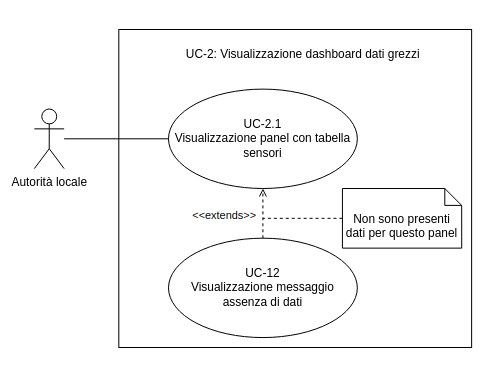
\includegraphics[width=0.75\textwidth]{analisi_dei_requisiti/UC-2.1.png}
	\captionof{figure}{UC-2.1: Visualizzazione grafico \href{https://7last.github.io/docs/rtb/documentazione-interna/glossario\#time-series}{time series\textsubscript{G}} per temperatura}
\end{center}

\subsubsubsection{UC-2.2: Visualizzazione mappa sensori temperatura}
\begin{itemize}
	\item \textbf{Attore principale}: Autorità locale;
	\item \textbf{Precondizioni}:
	      \begin{enumerate}
		      \item L'autorità locale ha effettuato l'accesso al sistema ed esso è in funzione;
		      \item Il sistema ha caricato la \href{https://7last.github.io/docs/rtb/documentazione-interna/glossario\#dashboard}{dashboard\textsubscript{G}} relativa ai sensori di temperatura;
	      \end{enumerate}
	\item \textbf{Postcondizioni}: L'autorità locale visualizza una mappa interattiva popolata con dei marker rappresentanti la posizione dei sensori di temperatura;
	\item \textbf{Scenario principale}:
	      \begin{enumerate}
		      \item L'autorità locale accede alla piattaforma;
		      \item Il sistema carica i dati relativi ai sensori interrogando il database;
		      \item L'autorità locale seleziona la visualizzazione della \href{https://7last.github.io/docs/rtb/documentazione-interna/glossario\#dashboard}{dashboard\textsubscript{G}} relativa ai sensori di temperatura.
	      \end{enumerate}
	\item \href{https://7last.github.io/docs/rtb/documentazione-interna/glossario\#user-story}{\textbf{User story}\textsubscript{G}}:
	      Come autorità locale desidero poter visualizzare una mappa interattiva popolata con dei marker rappresentanti la posizione dei sensori di temperatura e contenenti il loro identificativo. Essa mi consentirà di visualizzare la distribuzione dei sensori di temperatura nel territorio ed eventualmente interventire nel caso in cui siano presenti zone non coperte.
\end{itemize}
\begin{center}
	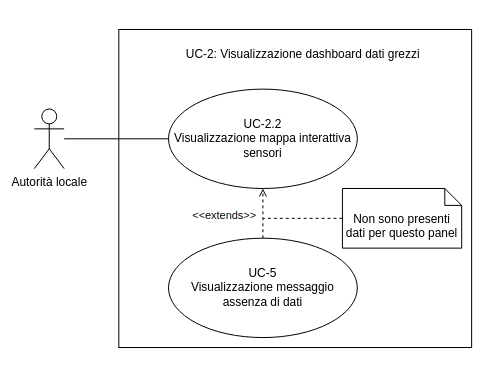
\includegraphics[width=0.75\textwidth]{analisi_dei_requisiti/UC-2.2.png}
	\captionof{figure}{UC-2.2: Visualizzazione mappa interattiva sensori temperatura}
\end{center}

\subsubsubsection{UC-2.3: Visualizzazione panel temperatura media in un determinato periodo di tempo}
\begin{itemize}
	\item \textbf{Attore principale}: Autorità locale;
	\item \textbf{Precondizioni}:
	      \begin{enumerate}
		      \item L'autorità locale ha effettuato l'accesso al sistema ed esso è in funzione;
		      \item Il sistema ha caricato la \href{https://7last.github.io/docs/rtb/documentazione-interna/glossario\#dashboard}{dashboard\textsubscript{G}} relativa ai sensori di temperatura;
	      \end{enumerate}
	\item \textbf{Postcondizioni}: L'autorità locale visualizza un \textit{panel} contenente la temperatura media in un determinato periodo di tempo;
	\item \textbf{Scenario principale}:
	      \begin{enumerate}
		      \item L'autorità locale accede alla piattaforma;
		      \item Il sistema carica i dati relativi ai sensori interrogando il database;
		      \item L'autorità locale seleziona la visualizzazione della \href{https://7last.github.io/docs/rtb/documentazione-interna/glossario\#dashboard}{dashboard\textsubscript{G}} relativa ai sensori di temperatura.
	      \end{enumerate}
	\item \href{https://7last.github.io/docs/rtb/documentazione-interna/glossario\#user-story}{\textbf{User story}\textsubscript{G}}: Come autorità locale desidero poter visualizzare la temperatura media in un determinato periodo di tempo
	      in modo da poterne monitorare l'andamento.
\end{itemize}
\begin{center}
	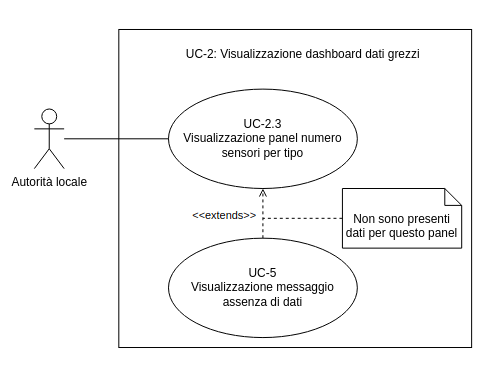
\includegraphics[width=0.75\textwidth]{analisi_dei_requisiti/UC-2.3.png}
	\captionof{figure}{UC-2.3: Visualizzazione \textit{panel} temperatura media in un determinato periodo di tempo}
\end{center}

\subsubsubsection{UC-2.4: Visualizzazione panel temperatura in tempo reale}
\begin{itemize}
	\item \textbf{Attore principale}: Autorità locale;
	\item \textbf{Precondizioni}:
	      \begin{enumerate}
		      \item L'autorità locale ha effettuato l'accesso al sistema ed esso è in funzione;
		      \item Il sistema ha caricato la \href{https://7last.github.io/docs/rtb/documentazione-interna/glossario\#dashboard}{dashboard\textsubscript{G}} relativa ai sensori di temperatura;
	      \end{enumerate}
	\item \textbf{Postcondizioni}: L'autorità locale visualizza un \textit{panel} contenente la temperatura in tempo reale;
	\item \textbf{Scenario principale}:
	      \begin{enumerate}
		      \item L'autorità locale accede alla piattaforma;
		      \item Il sistema carica i dati relativi ai sensori interrogando il database;
		      \item L'autorità locale seleziona la visualizzazione della \href{https://7last.github.io/docs/rtb/documentazione-interna/glossario\#dashboard}{dashboard\textsubscript{G}} relativa ai sensori di temperatura.
	      \end{enumerate}
	\item \href{https://7last.github.io/docs/rtb/documentazione-interna/glossario\#user-story}{\textbf{User story}\textsubscript{G}}:
	      Come autorità locale desidero poter visualizzare la temperatura in tempo reale in modo da poterne monitorare l'andamento
	      e poterla facilmente confrontare con i dati storici.
\end{itemize}
\begin{center}
	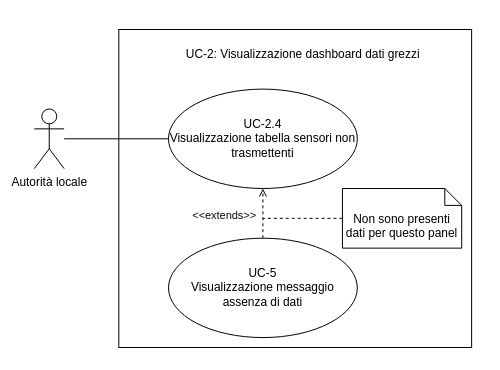
\includegraphics[width=0.75\textwidth]{analisi_dei_requisiti/UC-2.4.png}
	\captionof{figure}{UC-2.4: Visualizzazione \textit{panel} temperatura in tempo reale}
\end{center}

\subsubsubsection{UC-2.5: Visualizzazione panel temperatura massima in un determinato periodo di tempo}
\begin{itemize}
	\item \textbf{Attore principale}: Autorità locale;
	\item \textbf{Precondizioni}:
	      \begin{enumerate}
		      \item L'autorità locale ha effettuato l'accesso al sistema ed esso è in funzione;
		      \item Il sistema ha caricato la \href{https://7last.github.io/docs/rtb/documentazione-interna/glossario\#dashboard}{dashboard\textsubscript{G}} relativa ai sensori di temperatura;
	      \end{enumerate}
	\item \textbf{Postcondizioni}: L'autorità locale visualizza un \textit{panel} contenente la temperatura massima in un determinato periodo di tempo;
	\item \textbf{Scenario principale}:
	      \begin{enumerate}
		      \item L'autorità locale accede alla piattaforma;
		      \item Il sistema carica i dati relativi ai sensori interrogando il database;
		      \item L'autorità locale seleziona la visualizzazione della \href{https://7last.github.io/docs/rtb/documentazione-interna/glossario\#dashboard}{dashboard\textsubscript{G}} relativa ai sensori di temperatura.
	      \end{enumerate}
	\item \href{https://7last.github.io/docs/rtb/documentazione-interna/glossario\#user-story}{\textbf{User story}\textsubscript{G}}:
	      Come autorità locale desidero poter visualizzare la temperatura massima in un determinato periodo di tempo
	      in modo da poterla prendere come riferimento e confrontarla con la temperatura attuale.
\end{itemize}
\begin{center}
	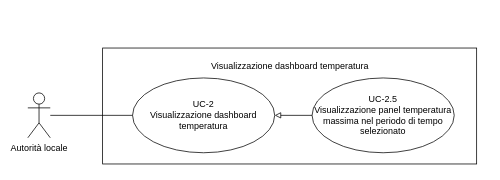
\includegraphics[width=0.75\textwidth]{analisi_dei_requisiti/UC-2.5.png}
	\captionof{figure}{UC-2.5: Visualizzazione \textit{panel} temperatura massima}
\end{center}

\subsubsubsection{UC-2.6: Visualizzazione panel temperatura minima in un determinato periodo di tempo}
\begin{itemize}
	\item \textbf{Attore principale}: Autorità locale;
	\item \textbf{Precondizioni}:
	      \begin{enumerate}
		      \item L'autorità locale ha effettuato l'accesso al sistema ed esso è in funzione;
		      \item Il sistema ha caricato la \href{https://7last.github.io/docs/rtb/documentazione-interna/glossario\#dashboard}{dashboard\textsubscript{G}} relativa ai sensori di temperatura;
	      \end{enumerate}
	\item \textbf{Postcondizioni}: L'autorità locale visualizza un \textit{panel} contenente la temperatura minima in un determinato periodo di tempo;
	      \begin{enumerate}
		      \item L'autorità locale ha effettuato l'accesso al sistema ed esso è in funzione;
		      \item Il sistema ha caricato la \href{https://7last.github.io/docs/rtb/documentazione-interna/glossario\#dashboard}{dashboard\textsubscript{G}} relativa ai sensori di temperatura;
	      \end{enumerate}
	\item \textbf{Postcondizioni}: L'autorità locale visualizza un \textit{panel} contenente la temperatura minima in un determinato periodo di tempo;
	\item \textbf{Scenario principale}:
	      \begin{enumerate}
		      \item L'autorità locale accede alla piattaforma;
		      \item Il sistema carica i dati relativi ai sensori interrogando il database;
		      \item L'autorità locale seleziona la visualizzazione della \href{https://7last.github.io/docs/rtb/documentazione-interna/glossario\#dashboard}{dashboard\textsubscript{G}} relativa ai sensori di temperatura.
	      \end{enumerate}
	\item \href{https://7last.github.io/docs/rtb/documentazione-interna/glossario\#user-story}{\textbf{User story}\textsubscript{G}}:
	      Come autorità locale desidero poter visualizzare la temperatura minima in un determinato periodo di tempo
	      in modo da poterla prendere come riferimento e confrontarla con la temperatura attuale.
\end{itemize}
\begin{center}
	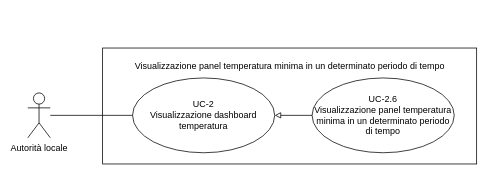
\includegraphics[width=0.75\textwidth]{analisi_dei_requisiti/UC-2.6.png}
	\captionof{figure}{UC-2.6: Visualizzazione \textit{panel} temperatura minima}
\end{center}

\subsubsection{UC-3: Visualizzazione dashboard umidità}
\begin{itemize}
	\item \textbf{Attore principale}: Autorità locale;
	\item \textbf{Precondizioni}: L'autorità locale ha effettuato l'accesso al sistema ed esso è in funzione;
	\item \textbf{Postcondizioni}: L'autorità locale visualizza la \href{https://7last.github.io/docs/rtb/documentazione-interna/glossario\#dashboard}{dashboard\textsubscript{G}} relativa
	      ai sensori di umidità presenti nella città;
	\item \textbf{Scenario principale}:
	      \begin{enumerate}
		      \item L'autorità locale accede alla piattaforma;
		      \item Il sistema carica i dati trasmessi dai sensori interrogando il database;
		      \item L'autorità locale seleziona la visualizzazione della \href{https://7last.github.io/docs/rtb/documentazione-interna/glossario\#dashboard}{dashboard\textsubscript{G}} relativa ai sensori di umidità.
	      \end{enumerate}
	\item \href{https://7last.github.io/docs/rtb/documentazione-interna/glossario\#user-story}{\textbf{User story}\textsubscript{G}}:
	      Come autorità locale desidero poter visualizzare una \href{https://7last.github.io/docs/rtb/documentazione-interna/glossario\#dashboard}{dashboard\textsubscript{G}} relativa ai sensori di umidità presenti nella città, la quale
	      dovrà contenere informazioni utili per monitorare l'andamento dell'umidità sulla base di dati storici e in tempo reale, mostrando
	      anche statistiche quali l'umidità media, massima e minima in un determinato periodo di tempo.
\end{itemize}
\begin{center}
	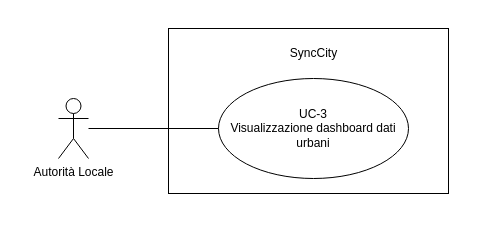
\includegraphics[width=0.6\textwidth]{analisi_dei_requisiti/UC-3.png}
	\captionof{figure}{UC-3: Visualizzazione \href{https://7last.github.io/docs/rtb/documentazione-interna/glossario\#dashboard}{dashboard\textsubscript{G}} umidità}
\end{center}

\subsubsubsection{UC-3.1: Visualizzazione grafico time series umidità}
\begin{itemize}
	\item \textbf{Attore principale}: Autorità locale;
	\item \textbf{Precondizioni}:
	      \begin{enumerate}
		      \item L'autorità locale ha effettuato l'accesso al sistema ed esso è in funzione;
		      \item Il sistema ha caricato la \href{https://7last.github.io/docs/rtb/documentazione-interna/glossario\#dashboard}{dashboard\textsubscript{G}} relativa ai sensori di umidità
	      \end{enumerate}
	\item \textbf{Postcondizioni}: L'autorità locale visualizza un grafico \href{https://7last.github.io/docs/rtb/documentazione-interna/glossario\#time-series}{time series\textsubscript{G}} contenente le misurazioni storiche
	      di umidità;
	\item \textbf{Scenario principale}:
	      \begin{enumerate}
		      \item L'autorità locale accede alla piattaforma;
		      \item Il sistema carica i dati relativi ai sensori interrogando il database;
		      \item L'autorità locale seleziona la visualizzazione della \href{https://7last.github.io/docs/rtb/documentazione-interna/glossario\#dashboard}{dashboard\textsubscript{G}} relativa ai sensori di umidità;
	      \end{enumerate}
	\item \href{https://7last.github.io/docs/rtb/documentazione-interna/glossario\#user-story}{\textbf{User story}\textsubscript{G}}:
	      Come autorità locale desidero poter visualizzare un grafico \href{https://7last.github.io/docs/rtb/documentazione-interna/glossario\#time-series}{time series\textsubscript{G}} contenente le misurazioni storiche
	      di umidità per poter monitorarne l'andamento nel tempo e facilmente individuare eventuali anomalie.
\end{itemize}
\begin{center}
	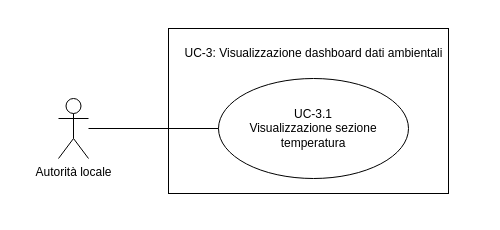
\includegraphics[width=0.75\textwidth]{analisi_dei_requisiti/UC-3.1.png}
	\captionof{figure}{UC-3.1, Visualizzazione grafico \href{https://7last.github.io/docs/rtb/documentazione-interna/glossario\#time-series}{time series\textsubscript{G}} umidità}
\end{center}

\subsubsubsection{UC-3.2: Visualizzazione mappa sensori umidità}
\begin{itemize}
	\item \textbf{Attore principale}: Autorità locale;
	\item \textbf{Precondizioni}:
	      \begin{enumerate}
		      \item L'autorità locale ha effettuato l'accesso al sistema ed esso è in funzione;
		      \item Il sistema ha caricato la \href{https://7last.github.io/docs/rtb/documentazione-interna/glossario\#dashboard}{dashboard\textsubscript{G}} relativa ai sensori di umidità;
	      \end{enumerate}
	\item \textbf{Postcondizioni}: L'autorità locale visualizza una mappa interattiva popolata con dei marker rappresentanti la posizione dei sensori di umidità;
	\item \textbf{Scenario principale}:
	      \begin{enumerate}
		      \item L'autorità locale accede alla piattaforma;
		      \item Il sistema carica i dati relativi ai sensori interrogando il database;
		      \item L'autorità locale seleziona la visualizzazione della \href{https://7last.github.io/docs/rtb/documentazione-interna/glossario\#dashboard}{dashboard\textsubscript{G}} relativa ai sensori di umidità.
	      \end{enumerate}
	\item \href{https://7last.github.io/docs/rtb/documentazione-interna/glossario\#user-story}{\textbf{User story}\textsubscript{G}}:
	      Come autorità locale desidero poter visualizzare una mappa interattiva popolata con dei marker rappresentanti la posizione dei sensori di umidità
	      e contenenti il loro identificativo. Essa mi consentirà di visualizzare la distribuzione dei sensori di umidità nel territorio ed eventualmente interventire nel caso in cui siano presenti zone non coperte.
\end{itemize}
\begin{center}
	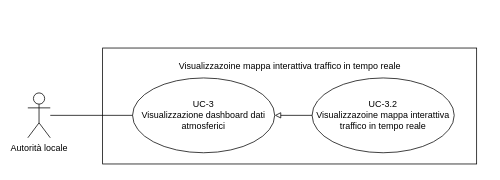
\includegraphics[width=0.75\textwidth]{analisi_dei_requisiti/UC-3.2.png}
	\captionof{figure}{UC-3.2: Visualizzazione mappa interattiva sensori umidità}
\end{center}

\subsubsubsection{UC-3.3: Visualizzazione panel umidità media in un determinato periodo di tempo}
\begin{itemize}
	\item \textbf{Attore principale}: Autorità locale;
	\item \textbf{Precondizioni}:
	      \begin{enumerate}
		      \item L'autorità locale ha effettuato l'accesso al sistema ed esso è in funzione;
		      \item Il sistema ha caricato la \href{https://7last.github.io/docs/rtb/documentazione-interna/glossario\#dashboard}{dashboard\textsubscript{G}} relativa ai sensori di umidità;
	      \end{enumerate}
	\item \textbf{Postcondizioni}: L'autorità locale visualizza un \textit{panel} contenente l'umidità media in un determinato periodo di tempo;
	\item \textbf{Scenario principale}:
	      \begin{enumerate}
		      \item L'autorità locale accede alla piattaforma;
		      \item Il sistema carica i dati relativi ai sensori interrogando il database;
		      \item L'autorità locale seleziona la visualizzazione della \href{https://7last.github.io/docs/rtb/documentazione-interna/glossario\#dashboard}{dashboard\textsubscript{G}} relativa ai sensori di umidità.
	      \end{enumerate}
	\item \href{https://7last.github.io/docs/rtb/documentazione-interna/glossario\#user-story}{\textbf{User story}\textsubscript{G}}: Come autorità locale desidero poter visualizzare l'umidità media in un determinato periodo di tempo
	      in modo da poterne monitorare l'andamento.
\end{itemize}
\begin{center}
	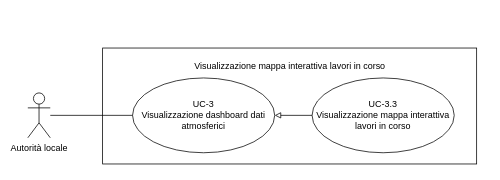
\includegraphics[width=0.75\textwidth]{analisi_dei_requisiti/UC-3.3.png}
	\captionof{figure}{UC-3.3: Visualizzazione \textit{panel} umidità media in un determinato periodo di tempo}
\end{center}

\subsubsubsection{UC-3.4: Visualizzazione panel umidità in tempo reale}
\begin{itemize}
	\item \textbf{Attore principale}: Autorità locale;
	\item \textbf{Precondizioni}:
	      \begin{enumerate}
		      \item L'autorità locale ha effettuato l'accesso al sistema ed esso è in funzione;
		      \item Il sistema ha caricato la \href{https://7last.github.io/docs/rtb/documentazione-interna/glossario\#dashboard}{dashboard\textsubscript{G}} relativa ai sensori di umidità;
	      \end{enumerate}
	\item \textbf{Postcondizioni}: L'autorità locale visualizza un \textit{panel} contenente l'umidità in tempo reale;
	\item \textbf{Scenario principale}:
	      \begin{enumerate}
		      \item L'autorità locale accede alla piattaforma;
		      \item Il sistema carica i dati relativi ai sensori interrogando il database;
		      \item L'autorità locale seleziona la visualizzazione della \href{https://7last.github.io/docs/rtb/documentazione-interna/glossario\#dashboard}{dashboard\textsubscript{G}} relativa ai sensori di umidità.
	      \end{enumerate}
	\item \href{https://7last.github.io/docs/rtb/documentazione-interna/glossario\#user-story}{\textbf{User story}\textsubscript{G}}:
	      Come autorità locale desidero poter visualizzare l'umidità in tempo reale in modo da poterne monitorare l'andamento
	      e poterla facilmente confrontare con i dati storici.
\end{itemize}
\begin{center}
	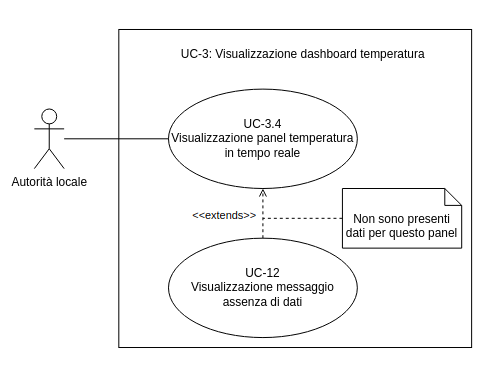
\includegraphics[width=0.75\textwidth]{analisi_dei_requisiti/UC-3.4.png}
	\captionof{figure}{UC-3.4: Visualizzazione \textit{panel} umidità in tempo reale}
\end{center}

\subsubsubsection{UC-3.5: Visualizzazione panel umidità massima in un determinato periodo di tempo}
\begin{itemize}
	\item \textbf{Attore principale}: Autorità locale;
	\item \textbf{Precondizioni}:
	      \begin{enumerate}
		      \item L'autorità locale ha effettuato l'accesso al sistema ed esso è in funzione;
		      \item Il sistema ha caricato la \href{https://7last.github.io/docs/rtb/documentazione-interna/glossario\#dashboard}{dashboard\textsubscript{G}} relativa ai sensori di umidità;
	      \end{enumerate}
	\item \textbf{Postcondizioni}: L'autorità locale visualizza un \textit{panel} contenente l'umidità massima in un determinato periodo di tempo;
	\item \textbf{Scenario principale}:
	      \begin{enumerate}
		      \item L'autorità locale accede alla piattaforma;
		      \item Il sistema carica i dati relativi ai sensori interrogando il database;
		      \item L'autorità locale seleziona la visualizzazione della \href{https://7last.github.io/docs/rtb/documentazione-interna/glossario\#dashboard}{dashboard\textsubscript{G}} relativa ai sensori di umidità.
	      \end{enumerate}
	\item \href{https://7last.github.io/docs/rtb/documentazione-interna/glossario\#user-story}{\textbf{User story}\textsubscript{G}}:
	      Come autorità locale desidero poter visualizzare l'umidità massima in un determinato periodo di tempo
	      in modo da poterla prendere come riferimento e confrontarla con l'umidità attuale.
\end{itemize}
\begin{center}
	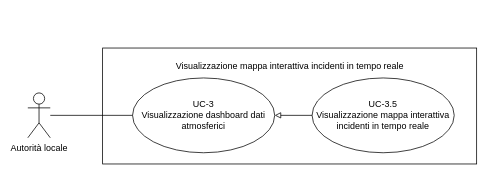
\includegraphics[width=0.75\textwidth]{analisi_dei_requisiti/UC-3.5.png}
	\captionof{figure}{UC-3.5: Visualizzazione \textit{panel} umidità massima}
\end{center}

\subsubsubsection{UC-3.6: Visualizzazione panel umidità minima in un determinato periodo di tempo}
\begin{itemize}
	\item \textbf{Attore principale}: Autorità locale;
	\item \textbf{Precondizioni}:
	      \begin{enumerate}
		      \item L'autorità locale ha effettuato l'accesso al sistema ed esso è in funzione;
		      \item Il sistema ha caricato la \href{https://7last.github.io/docs/rtb/documentazione-interna/glossario\#dashboard}{dashboard\textsubscript{G}} relativa ai sensori di umidità;
	      \end{enumerate}
	\item \textbf{Postcondizioni}: L'autorità locale visualizza un \textit{panel} contenente l'umidità minima in un determinato periodo di tempo;
	\item \textbf{Scenario principale}:
	      \begin{enumerate}
		      \item L'autorità locale accede alla piattaforma;
		      \item Il sistema carica i dati relativi ai sensori interrogando il database;
		      \item L'autorità locale seleziona la visualizzazione della \href{https://7last.github.io/docs/rtb/documentazione-interna/glossario\#dashboard}{dashboard\textsubscript{G}} relativa ai sensori di umidità.
	      \end{enumerate}
	\item \href{https://7last.github.io/docs/rtb/documentazione-interna/glossario\#user-story}{\textbf{User story}\textsubscript{G}}:
	      Come autorità locale desidero poter visualizzare l'umidità minima in un determinato periodo di tempo
	      in modo da poterla prendere come riferimento e confrontarla con l'umidità attuale.
\end{itemize}
\begin{center}
	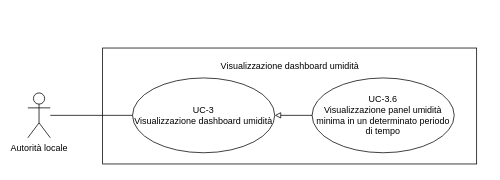
\includegraphics[width=0.75\textwidth]{analisi_dei_requisiti/UC-3.6.png}
	\captionof{figure}{UC-3.6: Visualizzazione \textit{panel} umidità minima}
\end{center}

\subsubsection{UC-4: Visualizzazione dashboard qualità dell'aria}
\begin{itemize}
	\item \textbf{Attore principale}: Autorità locale;
	\item \textbf{Precondizioni}: L'autorità locale ha effettuato l'accesso al sistema ed esso è in funzione;
	\item \textbf{Postcondizioni}: L'autorità locale visualizza la \href{https://7last.github.io/docs/rtb/documentazione-interna/glossario\#dashboard}{dashboard\textsubscript{G}} relativa
	      ai sensori di qualità dell'aria presenti nella città;
	\item \textbf{Scenario principale}:
	      \begin{enumerate}
		      \item L'autorità locale accede alla piattaforma;
		      \item Il sistema carica i dati trasmessi dai sensori interrogando il database;
		      \item L'autorità locale seleziona la visualizzazione della \href{https://7last.github.io/docs/rtb/documentazione-interna/glossario\#dashboard}{dashboard\textsubscript{G}} relativa ai sensori di qualità dell'aria.
	      \end{enumerate}
	\item \href{https://7last.github.io/docs/rtb/documentazione-interna/glossario\#user-story}{\textbf{User story}\textsubscript{G}}:
	      Come autorità locale desidero poter visualizzare una \href{https://7last.github.io/docs/rtb/documentazione-interna/glossario\#dashboard}{dashboard\textsubscript{G}} relativa ai sensori di qualità dell'aria presenti nella città, la quale
	      dovrà contenere informazioni utili per monitorare l'andamento della qualità dell'aria sulla base di dati storici e in tempo reale, mostrando
	      anche statistiche quali il giorno con la qualità dell'aria peggiore e il giorno con la qualità dell'aria migliore in un determinato periodo di tempo.
\end{itemize}
\begin{center}
	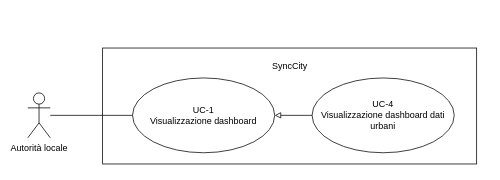
\includegraphics[width=0.6\textwidth]{analisi_dei_requisiti/UC-4.png}
	\captionof{figure}{UC-4: Visualizzazione \href{https://7last.github.io/docs/rtb/documentazione-interna/glossario\#dashboard}{dashboard\textsubscript{G}} qualità dell'aria}
\end{center}

\subsubsubsection{UC-4.1: Visualizzazione grafico time series qualità dell'aria}
\begin{itemize}
	\item \textbf{Attore principale}: Autorità locale;
	\item \textbf{Precondizioni}:
	      \begin{enumerate}
		      \item L'autorità locale ha effettuato l'accesso al sistema ed esso è in funzione;
		      \item Il sistema ha caricato la \href{https://7last.github.io/docs/rtb/documentazione-interna/glossario\#dashboard}{dashboard\textsubscript{G}} relativa ai sensori di qualità dell'aria
	      \end{enumerate}
	\item \textbf{Postcondizioni}: L'autorità locale visualizza un grafico \href{https://7last.github.io/docs/rtb/documentazione-interna/glossario\#time-series}{time series\textsubscript{G}} contenente le misurazioni storiche
	      di qualità dell'aria;
	\item \textbf{Scenario principale}:
	      \begin{enumerate}
		      \item L'autorità locale accede alla piattaforma;
		      \item Il sistema carica i dati relativi ai sensori interrogando il database;
		      \item L'autorità locale seleziona la visualizzazione della \href{https://7last.github.io/docs/rtb/documentazione-interna/glossario\#dashboard}{dashboard\textsubscript{G}} relativa ai sensori di qualità dell'aria;
	      \end{enumerate}
	\item \href{https://7last.github.io/docs/rtb/documentazione-interna/glossario\#user-story}{\textbf{User story}\textsubscript{G}}:
	      Come autorità locale desidero poter visualizzare un grafico \href{https://7last.github.io/docs/rtb/documentazione-interna/glossario\#time-series}{time series\textsubscript{G}} contenente le misurazioni storiche
	      di qualità dell'aria per poter monitorarne l'andamento nel tempo e facilmente individuare eventuali anomalie.
\end{itemize}
\begin{center}
	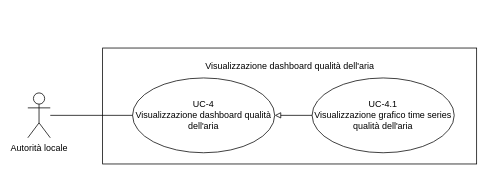
\includegraphics[width=0.75\textwidth]{analisi_dei_requisiti/UC-4.1.png}
	\captionof{figure}{UC-4.1, Visualizzazione grafico \href{https://7last.github.io/docs/rtb/documentazione-interna/glossario\#time-series}{time series\textsubscript{G}} qualità dell'aria}
\end{center}

\subsubsubsection{UC-4.2: Visualizzazione mappa interattiva sensori qualità dell'aria}
\begin{itemize}
	\item \textbf{Attore principale}: Autorità locale;
	\item \textbf{Precondizioni}:
	      \begin{enumerate}
		      \item L'autorità locale ha effettuato l'accesso al sistema ed esso è in funzione;
		      \item Il sistema ha caricato la \href{https://7last.github.io/docs/rtb/documentazione-interna/glossario\#dashboard}{dashboard\textsubscript{G}} relativa ai sensori di qualità dell'aria;
	      \end{enumerate}
	\item \textbf{Postcondizioni}: L'autorità locale visualizza una mappa interattiva popolata con dei marker rappresentanti la posizione dei sensori della qualità dell'aria;
	\item \textbf{Scenario principale}:
	      \begin{enumerate}
		      \item L'autorità locale accede alla piattaforma;
		      \item Il sistema carica i dati relativi ai sensori interrogando il database;
		      \item L'autorità locale seleziona la visualizzazione della \href{https://7last.github.io/docs/rtb/documentazione-interna/glossario\#dashboard}{dashboard\textsubscript{G}} relativa ai sensori della qualità dell'aria.
	      \end{enumerate}
	\item \href{https://7last.github.io/docs/rtb/documentazione-interna/glossario\#user-story}{\textbf{User story}\textsubscript{G}}:
	      Come autorità locale desidero poter visualizzare una mappa interattiva popolata con dei marker rappresentanti la posizione dei sensori della qualità dell'aria
	      e contenenti il loro identificativo. Essa mi consentirà di visualizzare la distribuzione dei sensori della qualità dell'aria nel territorio ed eventualmente interventire nel caso in cui siano presenti zone non coperte.
\end{itemize}
\begin{center}
	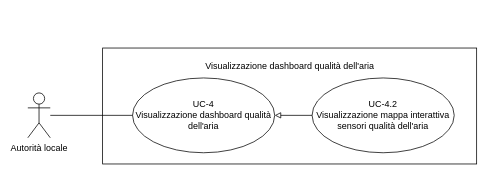
\includegraphics[width=0.75\textwidth]{analisi_dei_requisiti/UC-4.2.png}
	\captionof{figure}{UC-4.2: Visualizzazione mappa interattiva sensori qualità dell'aria}
\end{center}

\subsubsubsection{UC-4.3: Visualizzazione panel qualità dell'aria media in un determinato periodo di tempo}
\begin{itemize}
	\item \textbf{Attore principale}: Autorità locale;
	\item \textbf{Precondizioni}:
	      \begin{enumerate}
		      \item L'autorità locale ha effettuato l'accesso al sistema ed esso è in funzione;
		      \item Il sistema ha caricato la \href{https://7last.github.io/docs/rtb/documentazione-interna/glossario\#dashboard}{dashboard\textsubscript{G}} relativa ai sensori di qualità dell'aria;
	      \end{enumerate}
	\item \textbf{Postcondizioni}: L'autorità locale visualizza un \textit{panel} contenente qualità dell'aria media in un determinato periodo di tempo;
	\item \textbf{Scenario principale}:
	      \begin{enumerate}
		      \item L'autorità locale accede alla piattaforma;
		      \item Il sistema carica i dati relativi ai sensori interrogando il database;
		      \item L'autorità locale seleziona la visualizzazione della \href{https://7last.github.io/docs/rtb/documentazione-interna/glossario\#dashboard}{dashboard\textsubscript{G}} relativa ai sensori di qualità dell'aria.
	      \end{enumerate}
	\item \href{https://7last.github.io/docs/rtb/documentazione-interna/glossario\#user-story}{\textbf{User story}\textsubscript{G}}: Come autorità locale desidero poter visualizzare della qualità dell'aria media in un determinato periodo di tempo
	      in modo da poterne monitorare l'andamento.
\end{itemize}
\begin{center}
	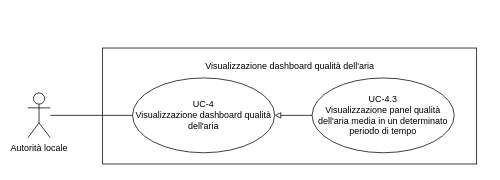
\includegraphics[width=0.75\textwidth]{analisi_dei_requisiti/UC-4.3.png}
	\captionof{figure}{UC-4.3: Visualizzazione \textit{panel} qualità dell'aria media in un determinato periodo di tempo}
\end{center}

\subsubsubsection{UC-4.4: Visualizzazione panel qualità dell'aria in tempo reale}
\begin{itemize}
	\item \textbf{Attore principale}: Autorità locale;
	\item \textbf{Precondizioni}:
	      \begin{enumerate}
		      \item L'autorità locale ha effettuato l'accesso al sistema ed esso è in funzione;
		      \item Il sistema ha caricato la \href{https://7last.github.io/docs/rtb/documentazione-interna/glossario\#dashboard}{dashboard\textsubscript{G}} relativa ai sensori di qualità dell'aria;
	      \end{enumerate}
	\item \textbf{Postcondizioni}: L'autorità locale visualizza un \textit{panel} contenente qualità dell'aria in tempo reale;
	\item \textbf{Scenario principale}:
	      \begin{enumerate}
		      \item L'autorità locale accede alla piattaforma;
		      \item Il sistema carica i dati relativi ai sensori interrogando il database;
		      \item L'autorità locale seleziona la visualizzazione della \href{https://7last.github.io/docs/rtb/documentazione-interna/glossario\#dashboard}{dashboard\textsubscript{G}} relativa ai sensori di qualità dell'aria.
	      \end{enumerate}
	\item \href{https://7last.github.io/docs/rtb/documentazione-interna/glossario\#user-story}{\textbf{User story}\textsubscript{G}}:
	      Come autorità locale desidero poter visualizzare della qualità dell'aria in tempo reale in modo da poterne monitorare l'andamento
	      e poterla facilmente confrontare con i dati storici.
\end{itemize}
\begin{center}
	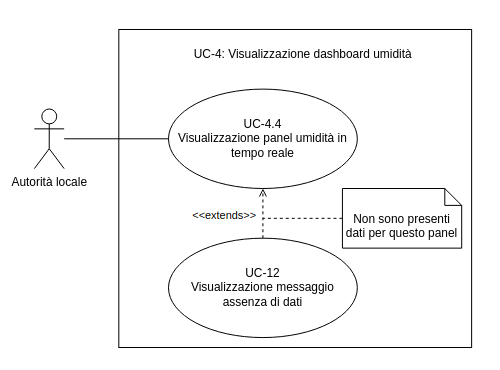
\includegraphics[width=0.75\textwidth]{analisi_dei_requisiti/UC-4.4.png}
	\captionof{figure}{UC-4.4: Visualizzazione \textit{panel} qualità dell'aria in tempo reale}
\end{center}
\subsubsubsection{UC-4.5: Visualizzazione panel giorno con qualità dell'aria peggiore in un determinato periodo di tempo}
\subsubsubsection{UC-4.6: Visualizzazione panel giorno con qualità dell'aria migliore in un determinato periodo di tempo}

\subsubsection{UC-5: Visualizzazione dashboard precipitazioni}
\begin{itemize}
	\item \textbf{Attore principale}: Autorità locale;
	\item \textbf{Precondizioni}: L'autorità locale ha effettuato l'accesso al sistema ed esso è in funzione;
	\item \textbf{Postcondizioni}: L'autorità locale visualizza la \href{https://7last.github.io/docs/rtb/documentazione-interna/glossario\#dashboard}{dashboard\textsubscript{G}} relativa
	      ai sensori di precipitazioni presenti nella città;
	\item \textbf{Scenario principale}:
	      \begin{enumerate}
		      \item L'autorità locale accede alla piattaforma;
		      \item Il sistema carica i dati trasmessi dai sensori interrogando il database;
		      \item L'autorità locale seleziona la visualizzazione della \href{https://7last.github.io/docs/rtb/documentazione-interna/glossario\#dashboard}{dashboard\textsubscript{G}} relativa ai sensori di precipitazioni.
	      \end{enumerate}
	\item \href{https://7last.github.io/docs/rtb/documentazione-interna/glossario\#user-story}{\textbf{User story}\textsubscript{G}}:
	      Come autorità locale desidero poter visualizzare una \href{https://7last.github.io/docs/rtb/documentazione-interna/glossario\#dashboard}{dashboard\textsubscript{G}} relativa ai sensori di precipitazioni presenti nella città, la quale
	      dovrà contenere informazioni utili per monitorare l'andamento dele precipitazioni sulla base di dati storici e in tempo reale, mostrando
	      anche statistiche quali quantità di precipitazioni media, massima e minima in un determinato periodo di tempo.
\end{itemize}
\begin{center}
	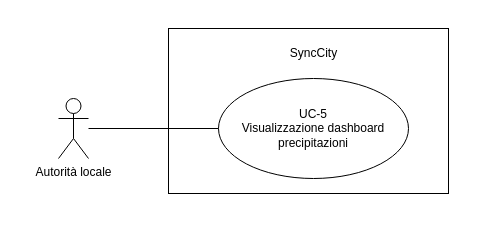
\includegraphics[width=0.6\textwidth]{analisi_dei_requisiti/UC-5.png}
	\captionof{figure}{UC-5: Visualizzazione \href{https://7last.github.io/docs/rtb/documentazione-interna/glossario\#dashboard}{dashboard\textsubscript{G}} precipitazioni}
\end{center}

\subsubsubsection{UC-5.1: Visualizzazione grafico time series quantità precipitazioni in un determinato periodo di tempo}
\begin{itemize}
	\item \textbf{Attore principale}: Autorità locale;
	\item \textbf{Precondizioni}:
	      \begin{enumerate}
		      \item L'autorità locale ha effettuato l'accesso al sistema ed esso è in funzione;
		      \item Il sistema ha caricato la \href{https://7last.github.io/docs/rtb/documentazione-interna/glossario\#dashboard}{dashboard\textsubscript{G}} relativa ai sensori di precipitazioni
	      \end{enumerate}
	\item \textbf{Postcondizioni}: L'autorità locale visualizza un grafico \href{https://7last.github.io/docs/rtb/documentazione-interna/glossario\#time-series}{time series\textsubscript{G}} contenente le misurazioni storiche
	      di precipitazioni;
	\item \textbf{Scenario principale}:
	      \begin{enumerate}
		      \item L'autorità locale accede alla piattaforma;
		      \item Il sistema carica i dati relativi ai sensori interrogando il database;
		      \item L'autorità locale seleziona la visualizzazione della \href{https://7last.github.io/docs/rtb/documentazione-interna/glossario\#dashboard}{dashboard\textsubscript{G}} relativa ai sensori di precipitazioni;
	      \end{enumerate}
	\item \href{https://7last.github.io/docs/rtb/documentazione-interna/glossario\#user-story}{\textbf{User story}\textsubscript{G}}:
	      Come autorità locale desidero poter visualizzare un grafico \href{https://7last.github.io/docs/rtb/documentazione-interna/glossario\#time-series}{time series\textsubscript{G}} contenente le misurazioni storiche
	      di precipitazioni per poter monitorarne l'andamento nel tempo e facilmente individuare eventuali anomalie.
\end{itemize}
\begin{center}
	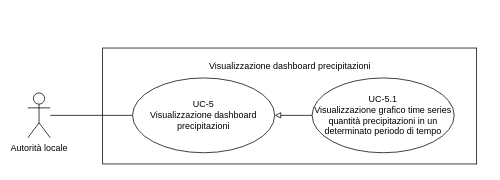
\includegraphics[width=0.75\textwidth]{analisi_dei_requisiti/UC-5.1.png}
	\captionof{figure}{UC-5.1, Visualizzazione grafico \href{https://7last.github.io/docs/rtb/documentazione-interna/glossario\#time-series}{time series\textsubscript{G}} precipitazioni}
\end{center}

\subsubsubsection{UC-5.2: Visualizzazione mappa sensori precipitazioni}
\begin{itemize}
	\item \textbf{Attore principale}: Autorità locale;
	\item \textbf{Precondizioni}:
	      \begin{enumerate}
		      \item L'autorità locale ha effettuato l'accesso al sistema ed esso è in funzione;
		      \item Il sistema ha caricato la \href{https://7last.github.io/docs/rtb/documentazione-interna/glossario\#dashboard}{dashboard\textsubscript{G}} relativa ai sensori di precipitazioni;
	      \end{enumerate}
	\item \textbf{Postcondizioni}: L'autorità locale visualizza una mappa interattiva popolata con dei marker rappresentanti la posizione dei sensori di precipitazioni;
	\item \textbf{Scenario principale}:
	      \begin{enumerate}
		      \item L'autorità locale accede alla piattaforma;
		      \item Il sistema carica i dati relativi ai sensori interrogando il database;
		      \item L'autorità locale seleziona la visualizzazione della \href{https://7last.github.io/docs/rtb/documentazione-interna/glossario\#dashboard}{dashboard\textsubscript{G}} relativa ai sensori di precipitazioni.
	      \end{enumerate}
	\item \href{https://7last.github.io/docs/rtb/documentazione-interna/glossario\#user-story}{\textbf{User story}\textsubscript{G}}:
	      Come autorità locale desidero poter visualizzare una mappa interattiva popolata con dei marker rappresentanti la posizione dei sensori di precipitazioni
	      e contenenti il loro identificativo. Essa mi consentirà di visualizzare la distribuzione dei sensori di precipitazioni nel territorio ed
	      eventualmente interventire nel caso in cui siano presenti zone non coperte.
\end{itemize}
\begin{center}
	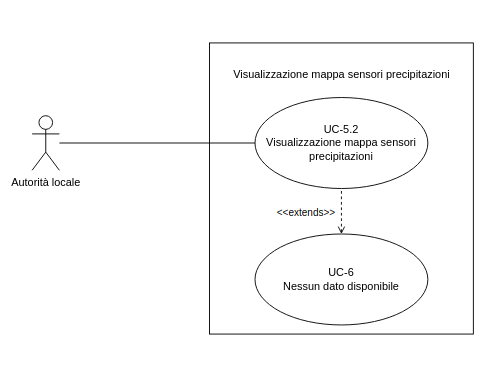
\includegraphics[width=0.75\textwidth]{analisi_dei_requisiti/UC-5.2.png}
	\captionof{figure}{UC-5.2: Visualizzazione mappa interattiva sensori precipitazioni}
\end{center}


\subsubsubsection{UC-5.3: Visualizzazione panel quantità di precipitazioni media in un determinato periodo di tempo}
\begin{itemize}
	\item \textbf{Attore principale}: Autorità locale;
	\item \textbf{Precondizioni}:
	      \begin{enumerate}
		      \item L'autorità locale ha effettuato l'accesso al sistema ed esso è in funzione;
		      \item Il sistema ha caricato la \href{https://7last.github.io/docs/rtb/documentazione-interna/glossario\#dashboard}{dashboard\textsubscript{G}} relativa ai sensori di quantità di precipitazioni;
	      \end{enumerate}
	\item \textbf{Postcondizioni}: L'autorità locale visualizza un \textit{panel} contenente di quantità di precipitazioni media in un determinato periodo di tempo;
	\item \textbf{Scenario principale}:
	      \begin{enumerate}
		      \item L'autorità locale accede alla piattaforma;
		      \item Il sistema carica i dati relativi ai sensori interrogando il database;
		      \item L'autorità locale seleziona la visualizzazione della \href{https://7last.github.io/docs/rtb/documentazione-interna/glossario\#dashboard}{dashboard\textsubscript{G}} relativa ai sensori di quantità di precipitazioni.
	      \end{enumerate}
	\item \href{https://7last.github.io/docs/rtb/documentazione-interna/glossario\#user-story}{\textbf{User story}\textsubscript{G}}: Come autorità locale desidero poter visualizzare di quantità di precipitazioni media in un determinato periodo di tempo
	      in modo da poterne monitorare l'andamento.
\end{itemize}
\begin{center}
	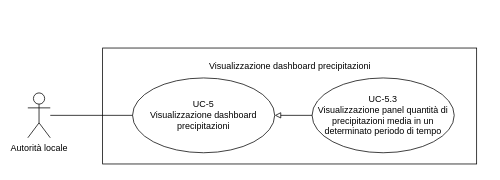
\includegraphics[width=0.75\textwidth]{analisi_dei_requisiti/UC-5.3.png}
	\captionof{figure}{UC-5.3: Visualizzazione \textit{panel} quantità di precipitazioni media in un determinato periodo di tempo}
\end{center}

\subsubsubsection{UC-5.4: Visualizzazione panel quantità di precipitazioni in tempo reale}
\begin{itemize}
	\item \textbf{Attore principale}: Autorità locale;
	\item \textbf{Precondizioni}:
	      \begin{enumerate}
		      \item L'autorità locale ha effettuato l'accesso al sistema ed esso è in funzione;
		      \item Il sistema ha caricato la \href{https://7last.github.io/docs/rtb/documentazione-interna/glossario\#dashboard}{dashboard\textsubscript{G}} relativa ai sensori di quantità di precipitazioni;
	      \end{enumerate}
	\item \textbf{Postcondizioni}: L'autorità locale visualizza un \textit{panel} contenente di quantità di precipitazioni in tempo reale;
	\item \textbf{Scenario principale}:
	      \begin{enumerate}
		      \item L'autorità locale accede alla piattaforma;
		      \item Il sistema carica i dati relativi ai sensori interrogando il database;
		      \item L'autorità locale seleziona la visualizzazione della \href{https://7last.github.io/docs/rtb/documentazione-interna/glossario\#dashboard}{dashboard\textsubscript{G}} relativa ai sensori di quantità di precipitazioni.
	      \end{enumerate}
	\item \href{https://7last.github.io/docs/rtb/documentazione-interna/glossario\#user-story}{\textbf{User story}\textsubscript{G}}:
	      Come autorità locale desidero poter visualizzare di quantità di precipitazioni in tempo reale in modo da poterne monitorare l'andamento
	      e poterla facilmente confrontare con i dati storici.
\end{itemize}
\begin{center}
	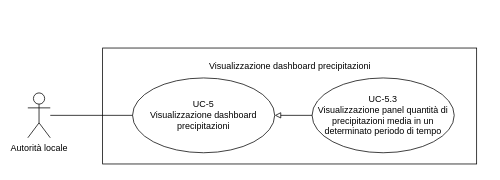
\includegraphics[width=0.75\textwidth]{analisi_dei_requisiti/UC-5.3.png}
	\captionof{figure}{UC-5.3: Visualizzazione \textit{panel} quantità di precipitazioni in tempo reale}
\end{center}

\subsubsubsection{UC-5.5: Visualizzazione panel giorno con precipitazioni maggiori in un determinato periodo di tempo}
\subsubsubsection{UC-5.6: Visualizzazione panel giorno con precipitazioni minori in un determinato periodo di tempo}

\subsubsection{UC-6: Visualizzazione dashboard traffico}
\begin{itemize}
	\item \textbf{Attore principale}: Autorità locale;
	\item \textbf{Precondizioni}: L'autorità locale ha effettuato l'accesso al sistema ed esso è in funzione;
	\item \textbf{Postcondizioni}: L'autorità locale visualizza la \href{https://7last.github.io/docs/rtb/documentazione-interna/glossario\#dashboard}{dashboard\textsubscript{G}} relativa
	      ai sensori di traffico presenti nella città;
	\item \textbf{Scenario principale}:
	      \begin{enumerate}
		      \item L'autorità locale accede alla piattaforma;
		      \item Il sistema carica i dati trasmessi dai sensori interrogando il database;
		      \item L'autorità locale seleziona la visualizzazione della \href{https://7last.github.io/docs/rtb/documentazione-interna/glossario\#dashboard}{dashboard\textsubscript{G}} relativa ai sensori di traffico.
	      \end{enumerate}
	\item \href{https://7last.github.io/docs/rtb/documentazione-interna/glossario\#user-story}{\textbf{User story}\textsubscript{G}}:
	      Come autorità locale desidero poter visualizzare una \href{https://7last.github.io/docs/rtb/documentazione-interna/glossario\#dashboard}{dashboard\textsubscript{G}} relativa ai sensori di traffico presenti nella città, la quale
	      dovrà contenere informazioni utili per monitorare l'andamento del traffico sulla base di dati storici e in tempo reale, mostrando
	      anche statistiche quali numero di veicoli in tempo reale, velocità media in tempo reale e calcolo dell'ora di punta (basato su numero veicoli e velocità media).
\end{itemize}
\begin{center}
	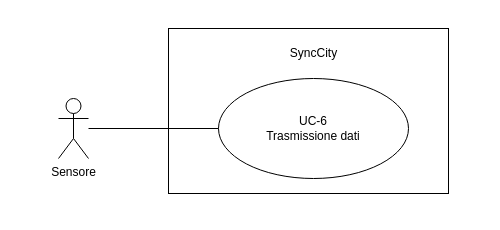
\includegraphics[width=0.6\textwidth]{analisi_dei_requisiti/UC-6.png}
	\captionof{figure}{UC-6: Visualizzazione \href{https://7last.github.io/docs/rtb/documentazione-interna/glossario\#dashboard}{dashboard\textsubscript{G}} traffico}
\end{center}

\subsubsubsection{UC-6.1: Visualizzazione grafico time series traffico}
\begin{itemize}
	\item \textbf{Attore principale}: Autorità locale;
	\item \textbf{Precondizioni}:
	      \begin{enumerate}
		      \item L'autorità locale ha effettuato l'accesso al sistema ed esso è in funzione;
		      \item Il sistema ha caricato la \href{https://7last.github.io/docs/rtb/documentazione-interna/glossario\#dashboard}{dashboard\textsubscript{G}} relativa ai sensori di traffico
	      \end{enumerate}
	\item \textbf{Postcondizioni}: L'autorità locale visualizza un grafico \href{https://7last.github.io/docs/rtb/documentazione-interna/glossario\#time-series}{time series\textsubscript{G}} contenente le misurazioni storiche
	      di traffico;
	\item \textbf{Scenario principale}:
	      \begin{enumerate}
		      \item L'autorità locale accede alla piattaforma;
		      \item Il sistema carica i dati relativi ai sensori interrogando il database;
		      \item L'autorità locale seleziona la visualizzazione della \href{https://7last.github.io/docs/rtb/documentazione-interna/glossario\#dashboard}{dashboard\textsubscript{G}} relativa ai sensori di traffico;
	      \end{enumerate}
	\item \href{https://7last.github.io/docs/rtb/documentazione-interna/glossario\#user-story}{\textbf{User story}\textsubscript{G}}:
	      Come autorità locale desidero poter visualizzare un grafico \href{https://7last.github.io/docs/rtb/documentazione-interna/glossario\#time-series}{time series\textsubscript{G}} contenente le misurazioni storiche
	      di traffico per poter monitorarne l'andamento nel tempo e facilmente individuare eventuali anomalie
	      o congestioni.
\end{itemize}
\begin{center}
	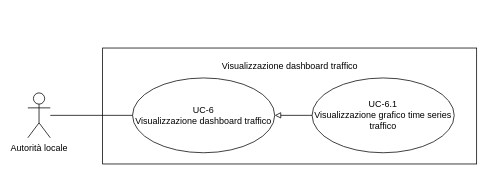
\includegraphics[width=0.75\textwidth]{analisi_dei_requisiti/UC-6.1.png}
	\captionof{figure}{UC-6.1, Visualizzazione grafico \href{https://7last.github.io/docs/rtb/documentazione-interna/glossario\#time-series}{time series\textsubscript{G}} traffico}
\end{center}

\subsubsubsection{UC-6.2: Visualizzazione mappa sensori traffico}
\begin{itemize}
	\item \textbf{Attore principale}: Autorità locale;
	\item \textbf{Precondizioni}:
	      \begin{enumerate}
		      \item L'autorità locale ha effettuato l'accesso al sistema ed esso è in funzione;
		      \item Il sistema ha caricato la \href{https://7last.github.io/docs/rtb/documentazione-interna/glossario\#dashboard}{dashboard\textsubscript{G}} relativa ai sensori di traffico;
	      \end{enumerate}
	\item \textbf{Postcondizioni}: L'autorità locale visualizza una mappa interattiva popolata con dei marker rappresentanti la posizione dei sensori del traffico;
	\item \textbf{Scenario principale}:
	      \begin{enumerate}
		      \item L'autorità locale accede alla piattaforma;
		      \item Il sistema carica i dati relativi ai sensori interrogando il database;
		      \item L'autorità locale seleziona la visualizzazione della \href{https://7last.github.io/docs/rtb/documentazione-interna/glossario\#dashboard}{dashboard\textsubscript{G}} relativa ai sensori del traffico.
	      \end{enumerate}
	\item \href{https://7last.github.io/docs/rtb/documentazione-interna/glossario\#user-story}{\textbf{User story}\textsubscript{G}}:
	      Come autorità locale desidero poter visualizzare una mappa interattiva popolata con dei marker rappresentanti la posizione dei sensori del traffico
	      e contenenti il loro identificativo. Essa mi consentirà di visualizzare la distribuzione dei sensori del traffico nel territorio ed eventualmente interventire nel caso in cui siano presenti zone non coperte.
\end{itemize}
\begin{center}
	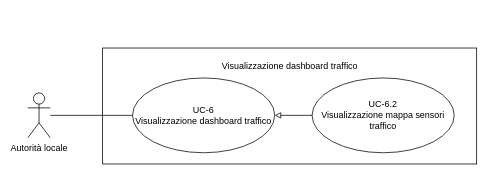
\includegraphics[width=0.75\textwidth]{analisi_dei_requisiti/UC-6.2.png}
	\captionof{figure}{UC-6.2: Visualizzazione mappa interattiva sensori traffico}
\end{center}

\subsubsubsection{UC-6.3: Visualizzazione panel numero veicoli in tempo reale}
\begin{itemize}
	\item \textbf{Attore principale}: Autorità locale;
	\item \textbf{Precondizioni}:
	      \begin{enumerate}
		      \item L'autorità locale ha effettuato l'accesso al sistema ed esso è in funzione;
		      \item Il sistema ha caricato la \href{https://7last.github.io/docs/rtb/documentazione-interna/glossario\#dashboard}{dashboard\textsubscript{G}} relativa ai sensori di traffico;
	      \end{enumerate}
	\item \textbf{Postcondizioni}: L'autorità locale visualizza un \textit{panel} contenente il numero di veicoli in tempo reale;
	\item \textbf{Scenario principale}:
	      \begin{enumerate}
		      \item L'autorità locale accede alla piattaforma;
		      \item Il sistema carica i dati relativi ai sensori interrogando il database;
		      \item L'autorità locale seleziona la visualizzazione della \href{https://7last.github.io/docs/rtb/documentazione-interna/glossario\#dashboard}{dashboard\textsubscript{G}} relativa ai sensori di traffico.
	      \end{enumerate}
	\item \href{https://7last.github.io/docs/rtb/documentazione-interna/glossario\#user-story}{\textbf{User story}\textsubscript{G}}:
	      Come autorità locale desidero poter visualizzare del numero di veicoli in tempo reale in modo da poterne monitorare l'andamento
	      e poterla facilmente confrontare con i dati storici.
\end{itemize}
\begin{center}
	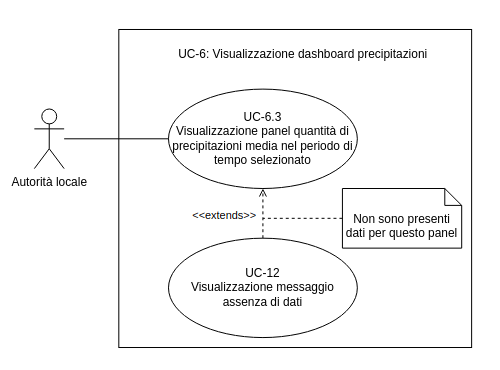
\includegraphics[width=0.75\textwidth]{analisi_dei_requisiti/UC-6.3.png}
	\captionof{figure}{UC-6.3: Visualizzazione \textit{panel} numero di veicoli in tempo reale}
\end{center}

\subsubsubsection{UC-6.4: Visualizzazione panel velocità media in tempo reale}
\begin{itemize}
	\item \textbf{Attore principale}: Autorità locale;
	\item \textbf{Precondizioni}:
	      \begin{enumerate}
		      \item L'autorità locale ha effettuato l'accesso al sistema ed esso è in funzione;
		      \item Il sistema ha caricato la \href{https://7last.github.io/docs/rtb/documentazione-interna/glossario\#dashboard}{dashboard\textsubscript{G}} relativa ai sensori di traffico;
	      \end{enumerate}
	\item \textbf{Postcondizioni}: L'autorità locale visualizza un \textit{panel} contenente la velocità media in tempo reale;
	\item \textbf{Scenario principale}:
	      \begin{enumerate}
		      \item L'autorità locale accede alla piattaforma;
		      \item Il sistema carica i dati relativi ai sensori interrogando il database;
		      \item L'autorità locale seleziona la visualizzazione della \href{https://7last.github.io/docs/rtb/documentazione-interna/glossario\#dashboard}{dashboard\textsubscript{G}} relativa ai sensori di traffico.
	      \end{enumerate}
	\item \href{https://7last.github.io/docs/rtb/documentazione-interna/glossario\#user-story}{\textbf{User story}\textsubscript{G}}:
	      Come autorità locale desidero poter visualizzare della velocità media in tempo reale in modo da poterne monitorare l'andamento
	      e poterla facilmente confrontare con i dati storici.
\end{itemize}
\begin{center}
	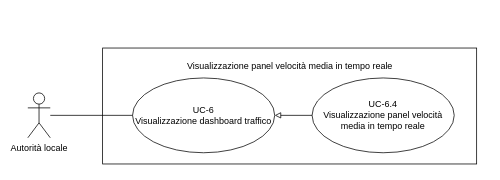
\includegraphics[width=0.75\textwidth]{analisi_dei_requisiti/UC-6.4.png}
	\captionof{figure}{UC-6.4: Visualizzazione \textit{panel} velocità media in tempo reale}
\end{center}

\subsubsubsection{UC-6.5: Visualizzazione panel calcolo ora di punta (numero veicoli e velocità media)}

\subsubsection{UC-7: Visualizzazione dashboard colonnine di ricarica}
\begin{itemize}
	\item \textbf{Attore principale}: Autorità locale;
	\item \textbf{Precondizioni}: L'autorità locale ha effettuato l'accesso al sistema ed esso è in funzione;
	\item \textbf{Postcondizioni}: L'autorità locale visualizza la \href{https://7last.github.io/docs/rtb/documentazione-interna/glossario\#dashboard}{dashboard\textsubscript{G}} relativa
	      alle colonnine di ricarica presenti nella città;
	\item \textbf{Scenario principale}:
	      \begin{enumerate}
		      \item L'autorità locale accede alla piattaforma;
		      \item Il sistema carica i dati trasmessi dai sensori interrogando il database;
		      \item L'autorità locale seleziona la visualizzazione della \href{https://7last.github.io/docs/rtb/documentazione-interna/glossario\#dashboard}{dashboard\textsubscript{G}} relativa alle colonnine di ricarica.
	      \end{enumerate}
	\item \href{https://7last.github.io/docs/rtb/documentazione-interna/glossario\#user-story}{\textbf{User story}\textsubscript{G}}:
	      Come autorità locale desidero poter visualizzare una \href{https://7last.github.io/docs/rtb/documentazione-interna/glossario\#dashboard}{dashboard\textsubscript{G}} relativa alle colonnine di ricarica presenti nella città, la quale
	      dovrà contenere informazioni riguro il loro stato di funzionamento e manutenzione.
\end{itemize}
\begin{center}
	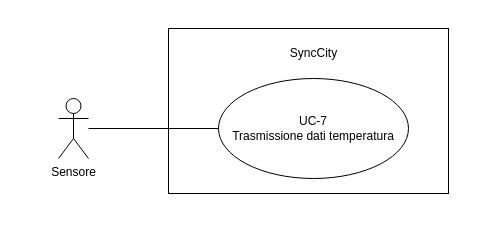
\includegraphics[width=0.6\textwidth]{analisi_dei_requisiti/UC-7.png}
	\captionof{figure}{UC-7: Visualizzazione \href{https://7last.github.io/docs/rtb/documentazione-interna/glossario\#dashboard}{dashboard\textsubscript{G}} colonnine di ricarica}
\end{center}

\subsubsubsection{UC-7.1: Visualizzazione mappa colonnine di ricarica con stato}
\begin{itemize}
	\item \textbf{Attore principale}: Autorità locale;
	\item \textbf{Precondizioni}:
	      \begin{enumerate}
		      \item L'autorità locale ha effettuato l'accesso al sistema ed esso è in funzione;
		      \item Il sistema ha caricato la \href{https://7last.github.io/docs/rtb/documentazione-interna/glossario\#dashboard}{dashboard\textsubscript{G}} relativa alle colonnine di ricarica;
	      \end{enumerate}
	\item \textbf{Postcondizioni}: L'autorità locale visualizza una mappa interattiva popolata con dei marker rappresentanti la posizione delle colonnine di ricarica;
	\item \textbf{Scenario principale}:
	      \begin{enumerate}
		      \item L'autorità locale accede alla piattaforma;
		      \item Il sistema carica i dati relativi ai sensori interrogando il database;
		      \item L'autorità locale seleziona la visualizzazione della \href{https://7last.github.io/docs/rtb/documentazione-interna/glossario\#dashboard}{dashboard\textsubscript{G}} relativa delle colonnine di ricarica.
	      \end{enumerate}
	\item \href{https://7last.github.io/docs/rtb/documentazione-interna/glossario\#user-story}{\textbf{User story}\textsubscript{G}}:
	      Come autorità locale desidero poter visualizzare una mappa interattiva popolata con dei marker rappresentanti la posizione delle colonnine di ricarica
	      contenenti il loro identificativo e lo stato di funzionamento. Essa mi consentirà di visualizzare la distribuzione delle colonnine di ricarica nel territorio
	      ed eventualmente interventire nel caso in cui vi siano dei guasti.
\end{itemize}
\begin{center}
	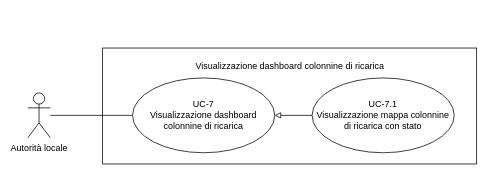
\includegraphics[width=0.75\textwidth]{analisi_dei_requisiti/UC-7.1.png}
	\captionof{figure}{UC-7.1: Visualizzazione mappa interattiva sensori colonnine di ricarica}
\end{center}

\subsubsubsection{UC-7.2: Visualizzazione panel numero colonnine di ricarica per stato in tempo reale}
\begin{itemize}
	\item \textbf{Attore principale}: Autorità locale;
	\item \textbf{Precondizioni}:
	      \begin{enumerate}
		      \item L'autorità locale ha effettuato l'accesso al sistema ed esso è in funzione;
		      \item Il sistema ha caricato la \href{https://7last.github.io/docs/rtb/documentazione-interna/glossario\#dashboard}{dashboard\textsubscript{G}} relativa ai \href{https://7last.github.io/docs/rtb/documentazione-interna/glossario\#dati-atmosferici}{dati atmosferici\textsubscript{G}};
	      \end{enumerate}
	\item \textbf{Postcondizioni}: L'autorità locale visualizza un \textit{panel} contenente il conteggio delle colonnine di ricarica suddivise per stato di funzionamento;
	\item \textbf{Scenario principale}:
	      \begin{enumerate}
		      \item L'autorità locale accede alla piattaforma;
		      \item Il sistema carica i dati relativi ai sensori interrogando il database;
		      \item L'autorità locale seleziona la visualizzazione della \href{https://7last.github.io/docs/rtb/documentazione-interna/glossario\#dashboard}{dashboard\textsubscript{G}} relativa alle colonnine di ricarica.
	      \end{enumerate}
	\item \href{https://7last.github.io/docs/rtb/documentazione-interna/glossario\#user-story}{\textbf{User story}\textsubscript{G}}:
	      Come autorità locale desidero poter visualizzare un \textit{panel} contenente il conteggio delle colonnine di ricarica suddivise per stato di funzionamento
	      per poterle monitorare e intervenire in caso di guasti.
\end{itemize}
\begin{center}
	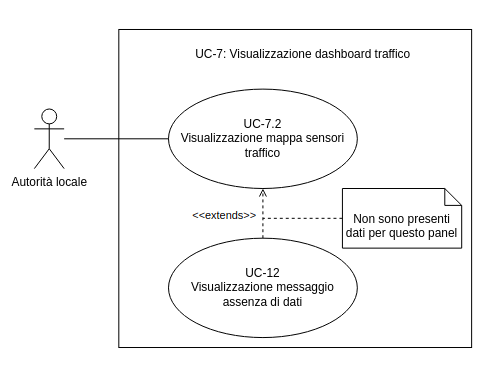
\includegraphics[width=0.6\textwidth]{analisi_dei_requisiti/UC-7.2.png}
	\captionof{figure}{UC-7.2: Visualizzazione \textit{panel} numero colonnine di ricarica per stato}
\end{center}

\subsubsection{UC-8: Visualizzazione dashboard parcheggi}
\begin{itemize}
	\item \textbf{Attore principale}: Autorità locale;
	\item \textbf{Precondizioni}: L'autorità locale ha effettuato l'accesso al sistema ed esso è in funzione;
	\item \textbf{Postcondizioni}: L'autorità locale visualizza la \href{https://7last.github.io/docs/rtb/documentazione-interna/glossario\#dashboard}{dashboard\textsubscript{G}} relativa
	      ai parcheggi presenti nella città;
	\item \textbf{Scenario principale}:
	      \begin{enumerate}
		      \item L'autorità locale accede alla piattaforma;
		      \item Il sistema carica i dati trasmessi dai sensori interrogando il database;
		      \item L'autorità locale seleziona la visualizzazione della \href{https://7last.github.io/docs/rtb/documentazione-interna/glossario\#dashboard}{dashboard\textsubscript{G}} relativa ai parcheggi.
	      \end{enumerate}
	\item \href{https://7last.github.io/docs/rtb/documentazione-interna/glossario\#user-story}{\textbf{User story}\textsubscript{G}}:
	      Come autorità locale desidero poter visualizzare una \href{https://7last.github.io/docs/rtb/documentazione-interna/glossario\#dashboard}{dashboard\textsubscript{G}} relativa ai parcheggi presenti nella città, la quale
	      dovrà contenere informazioni utili per monitorare lo stato di occupazione dei parcheggi sulla base di dati storici e in tempo reale,
	      in modo da poter individuare eventuali zone di criticità e intervenire per aumentare la disponibilità di parcheggi.
\end{itemize}
\begin{center}
	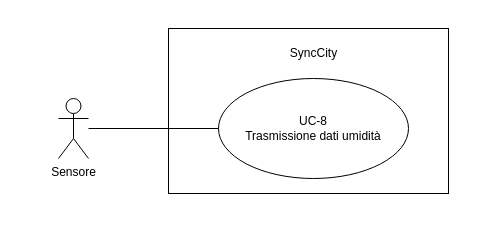
\includegraphics[width=0.6\textwidth]{analisi_dei_requisiti/UC-8.png}
	\captionof{figure}{UC-8: Visualizzazione \href{https://7last.github.io/docs/rtb/documentazione-interna/glossario\#dashboard}{dashboard\textsubscript{G}} parcheggi}
\end{center}

\subsubsubsection{UC-8.1: Visualizzazione mappa interattiva parcheggi con rispettivo stato di occupazione}
\begin{itemize}
	\item \textbf{Attore principale}: Autorità locale;
	\item \textbf{Precondizioni}:
	      \begin{enumerate}
		      \item L'autorità locale ha effettuato l'accesso al sistema ed esso è in funzione;
		      \item Il sistema ha caricato la \href{https://7last.github.io/docs/rtb/documentazione-interna/glossario\#dashboard}{dashboard\textsubscript{G}} relativa ai parcheggi con rispettivo stato di occupazione;
	      \end{enumerate}
	\item \textbf{Postcondizioni}: L'autorità locale visualizza una mappa interattiva popolata con dei marker rappresentanti la posizione dei parcheggi con rispettivo stato di occupazione;
	\item \textbf{Scenario principale}:
	      \begin{enumerate}
		      \item L'autorità locale accede alla piattaforma;
		      \item Il sistema carica i dati relativi ai sensori interrogando il database;
		      \item L'autorità locale seleziona la visualizzazione della \href{https://7last.github.io/docs/rtb/documentazione-interna/glossario\#dashboard}{dashboard\textsubscript{G}} relativa ai parcheggi.
	      \end{enumerate}
	\item \href{https://7last.github.io/docs/rtb/documentazione-interna/glossario\#user-story}{\textbf{User story}\textsubscript{G}}:
	      Come autorità locale desidero poter visualizzare una mappa interattiva popolata con dei marker rappresentanti la posizione dei parcheggi con rispettivo stato di occupazione
	      e contenenti il loro identificativo. Essa consentirà di individuare facilmente le zone con maggiore affluenza ed eventualmente intervenire per aumentare la disponibilità di parcheggi.
\end{itemize}
\begin{center}
	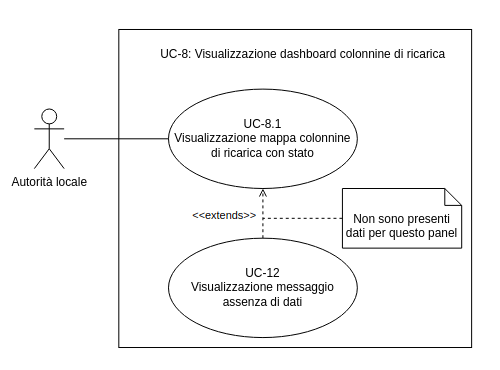
\includegraphics[width=0.75\textwidth]{analisi_dei_requisiti/UC-8.1.png}
	\captionof{figure}{UC-8.1: Visualizzazione mappa interattiva sensori parcheggi con rispettivo stato di occupazione}
\end{center}

\subsubsubsection{UC-8.2: Visualizzazione panel con conteggio parcheggi per stato in tempo reale}
\begin{itemize}
	\item \textbf{Attore principale}: Autorità locale;
	\item \textbf{Precondizioni}:
	      \begin{enumerate}
		      \item L'autorità locale ha effettuato l'accesso al sistema ed esso è in funzione;
		      \item Il sistema ha caricato la \href{https://7last.github.io/docs/rtb/documentazione-interna/glossario\#dashboard}{dashboard\textsubscript{G}} relativa ai parcheggi;
	      \end{enumerate}
	\item \textbf{Postcondizioni}: L'autorità locale visualizza un \textit{panel} contenente i parcheggi con rispettivo stato di occupazione in tempo reale;
	\item \textbf{Scenario principale}:
	      \begin{enumerate}
		      \item L'autorità locale accede alla piattaforma;
		      \item Il sistema carica i dati relativi ai sensori interrogando il database;
		      \item L'autorità locale seleziona la visualizzazione della \href{https://7last.github.io/docs/rtb/documentazione-interna/glossario\#dashboard}{dashboard\textsubscript{G}} relativa ai parcheggi con rispettivo stato di occupazione.
	      \end{enumerate}
	\item \href{https://7last.github.io/docs/rtb/documentazione-interna/glossario\#user-story}{\textbf{User story}\textsubscript{G}}:
	      Come autorità locale desidero poter visualizzare i parcheggi con rispettivo stato di occupazione in tempo reale in modo da poterne monitorare l'andamento
	      e poterla facilmente confrontare con i dati storici.
\end{itemize}
\begin{center}
	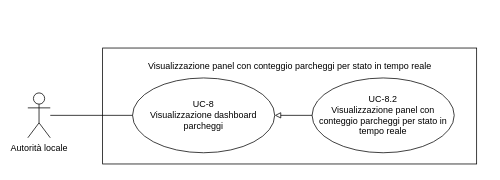
\includegraphics[width=0.75\textwidth]{analisi_dei_requisiti/UC-8.2.png}
	\captionof{figure}{UC-8.2: Visualizzazione \textit{panel} parcheggi con rispettivo stato di occupazione in tempo reale}
\end{center}

\subsubsection{UC-9: Visualizzazione dashboard isole ecologiche}
\begin{itemize}
	\item \textbf{Attore principale}: Autorità locale;
	\item \textbf{Precondizioni}: L'autorità locale ha effettuato l'accesso al sistema ed esso è in funzione;
	\item \textbf{Postcondizioni}: L'autorità locale visualizza la \href{https://7last.github.io/docs/rtb/documentazione-interna/glossario\#dashboard}{dashboard\textsubscript{G}} relativa
	      alle isole ecologiche presenti nella città;
	\item \textbf{Scenario principale}:
	      \begin{enumerate}
		      \item L'autorità locale accede alla piattaforma;
		      \item Il sistema carica i dati trasmessi dai sensori interrogando il database;
		      \item L'autorità locale seleziona la visualizzazione della \href{https://7last.github.io/docs/rtb/documentazione-interna/glossario\#dashboard}{dashboard\textsubscript{G}} relativa alle isole ecologiche.
	      \end{enumerate}
	\item \href{https://7last.github.io/docs/rtb/documentazione-interna/glossario\#user-story}{\textbf{User story}\textsubscript{G}}:
	      Come autorità locale desidero poter visualizzare una \href{https://7last.github.io/docs/rtb/documentazione-interna/glossario\#dashboard}{dashboard\textsubscript{G}} relativa alle isole ecologiche presenti nella città, la quale
	      dovrà contenere informazioni utili per monitorare il loro stato di riempimento. In questo modo potrò intervenire
	      per poter svuotare le isole ecologiche piene.
\end{itemize}
\begin{center}
	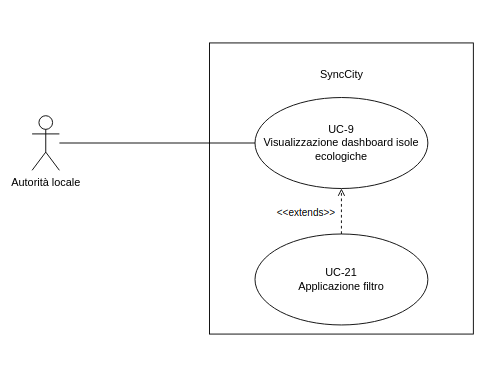
\includegraphics[width=0.6\textwidth]{analisi_dei_requisiti/UC-9.png}
	\captionof{figure}{UC-9: Visualizzazione \href{https://7last.github.io/docs/rtb/documentazione-interna/glossario\#dashboard}{dashboard\textsubscript{G}} isole ecologiche}
\end{center}

\subsubsubsection{UC-9.1: Visualizzazione panel con conteggio isole ecologiche piene in tempo reale}
\begin{itemize}
	\item \textbf{Attore principale}: Autorità locale;
	\item \textbf{Precondizioni}:
	      \begin{enumerate}
		      \item L'autorità locale ha effettuato l'accesso al sistema ed esso è in funzione;
		      \item Il sistema ha caricato la \href{https://7last.github.io/docs/rtb/documentazione-interna/glossario\#dashboard}{dashboard\textsubscript{G}} relativa alle isole ecologiche;
	      \end{enumerate}
	\item \textbf{Postcondizioni}: L'autorità locale visualizza un \textit{panel} contenente un conteggio delle isole ecologiche piene in tempo reale;
	\item \textbf{Scenario principale}:
	      \begin{enumerate}
		      \item L'autorità locale accede alla piattaforma;
		      \item Il sistema carica i dati relativi ai sensori interrogando il database;
		      \item L'autorità locale seleziona la visualizzazione della \href{https://7last.github.io/docs/rtb/documentazione-interna/glossario\#dashboard}{dashboard\textsubscript{G}} relativa alle isole ecologiche.
	      \end{enumerate}
	\item \href{https://7last.github.io/docs/rtb/documentazione-interna/glossario\#user-story}{\textbf{User story}\textsubscript{G}}:
	      Come autorità locale desidero poter visualizzare un conteggio delle isole ecologiche piene in tempo reale in modo da poter intervenire
	      per svuotarle.
\end{itemize}
\begin{center}
	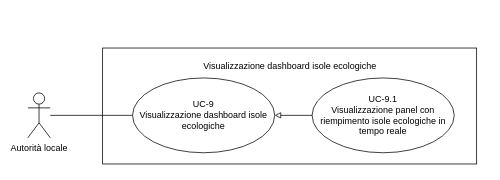
\includegraphics[width=0.75\textwidth]{analisi_dei_requisiti/UC-9.1.png}
	\captionof{figure}{UC-9.1: Visualizzazione \textit{panel} isole ecologiche piene in tempo reale}
\end{center}

\subsubsubsection{UC-9.2: Visualizzazione mappa interattiva isole ecologiche per stato di riempimento}
\begin{itemize}
	\item \textbf{Attore principale}: Autorità locale;
	\item \textbf{Precondizioni}:
	      \begin{enumerate}
		      \item L'autorità locale ha effettuato l'accesso al sistema ed esso è in funzione;
		      \item Il sistema ha caricato la \href{https://7last.github.io/docs/rtb/documentazione-interna/glossario\#dashboard}{dashboard\textsubscript{G}} relativa ai sensori di isole ecologiche;
	      \end{enumerate}
	\item \textbf{Postcondizioni}: L'autorità locale visualizza una mappa interattiva popolata con dei marker rappresentanti la posizione dei sensori delle isole ecologiche
	      suddivise per stato di riempimento;
	\item \textbf{Scenario principale}:
	      \begin{enumerate}
		      \item L'autorità locale accede alla piattaforma;
		      \item Il sistema carica i dati relativi ai sensori interrogando il database;
		      \item L'autorità locale seleziona la visualizzazione della \href{https://7last.github.io/docs/rtb/documentazione-interna/glossario\#dashboard}{dashboard\textsubscript{G}} relativa ai sensori delle isole ecologiche piene.
	      \end{enumerate}
	\item \href{https://7last.github.io/docs/rtb/documentazione-interna/glossario\#user-story}{\textbf{User story}\textsubscript{G}}:
	      Come autorità locale desidero poter visualizzare una mappa interattiva popolata con dei marker rappresentanti la posizione dei sensori delle isole ecologiche
	      suddivise per stato di riempimento e contenenti il loro identificativo.
	      Essa mi consentirà di visualizzare la distribuzione delle isole ecologiche nel territorio e di individuare facilmente quelle piene per poter intervenire e svuotarle.
\end{itemize}
\begin{center}
	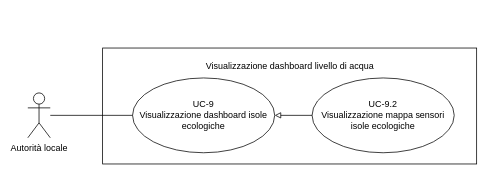
\includegraphics[width=0.75\textwidth]{analisi_dei_requisiti/UC-9.2.png}
	\captionof{figure}{UC-9.2: Visualizzazione mappa interattiva sensori isole ecologiche piene}
\end{center}

\subsubsection{UC-10: Visualizzazione dashboard livello di acqua}
\begin{itemize}
	\item \textbf{Attore principale}: Autorità locale;
	\item \textbf{Precondizioni}: L'autorità locale ha effettuato l'accesso al sistema ed esso è in funzione;
	\item \textbf{Postcondizioni}: L'autorità locale visualizza la \href{https://7last.github.io/docs/rtb/documentazione-interna/glossario\#dashboard}{dashboard\textsubscript{G}} relativa
	      ai sensori del livello di acqua presenti nella città;
	\item \textbf{Scenario principale}:
	      \begin{enumerate}
		      \item L'autorità locale accede alla piattaforma;
		      \item Il sistema carica i dati trasmessi dai sensori interrogando il database;
		      \item L'autorità locale seleziona la visualizzazione della \href{https://7last.github.io/docs/rtb/documentazione-interna/glossario\#dashboard}{dashboard\textsubscript{G}} relativa ai sensori del livello di acqua.
	      \end{enumerate}
	\item \href{https://7last.github.io/docs/rtb/documentazione-interna/glossario\#user-story}{\textbf{User story}\textsubscript{G}}:
	      Come autorità locale desidero poter visualizzare una \href{https://7last.github.io/docs/rtb/documentazione-interna/glossario\#dashboard}{dashboard\textsubscript{G}} relativa ai sensori del livello di acqua presenti nella città, la quale
	      dovrà contenere informazioni utili per monitorare il livello di acqua sulla base di dati storici e in tempo reale, mostrando
	      anche statistiche quali del livello di acqua medio in un determinato periodo di tempo e il livello di acqua in tempo reale.
\end{itemize}
\begin{center}
	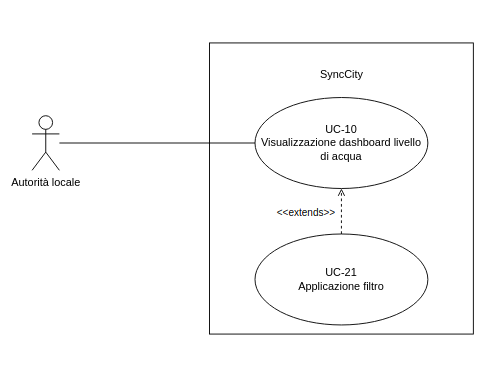
\includegraphics[width=0.6\textwidth]{analisi_dei_requisiti/UC-10.png}
	\captionof{figure}{UC-10: Visualizzazione \href{https://7last.github.io/docs/rtb/documentazione-interna/glossario\#dashboard}{dashboard\textsubscript{G}} livello di acqua}
\end{center}

\subsubsubsection{UC-10.1: Visualizzazione grafico time series livello di acqua}
\begin{itemize}
	\item \textbf{Attore principale}: Autorità locale;
	\item \textbf{Precondizioni}:
	      \begin{enumerate}
		      \item L'autorità locale ha effettuato l'accesso al sistema ed esso è in funzione;
		      \item Il sistema ha caricato la \href{https://7last.github.io/docs/rtb/documentazione-interna/glossario\#dashboard}{dashboard\textsubscript{G}} relativa ai sensori del livello di acqua.
	      \end{enumerate}
	\item \textbf{Postcondizioni}: L'autorità locale visualizza un grafico \href{https://7last.github.io/docs/rtb/documentazione-interna/glossario\#time-series}{time series\textsubscript{G}} contenente le misurazioni storiche
	      del livello di acqua;
	\item \textbf{Scenario principale}:
	      \begin{enumerate}
		      \item L'autorità locale accede alla piattaforma;
		      \item Il sistema carica i dati relativi ai sensori interrogando il database;
		      \item L'autorità locale seleziona la visualizzazione della \href{https://7last.github.io/docs/rtb/documentazione-interna/glossario\#dashboard}{dashboard\textsubscript{G}} relativa ai sensori del livello di acqua;
	      \end{enumerate}
	\item \href{https://7last.github.io/docs/rtb/documentazione-interna/glossario\#user-story}{\textbf{User story}\textsubscript{G}}:
	      Come autorità locale desidero poter visualizzare un grafico \href{https://7last.github.io/docs/rtb/documentazione-interna/glossario\#time-series}{time series\textsubscript{G}} contenente le misurazioni storiche
	      del livello di acqua per poter monitorarne l'andamento nel tempo e facilmente individuare eventuali anomalie.
\end{itemize}
\begin{center}
	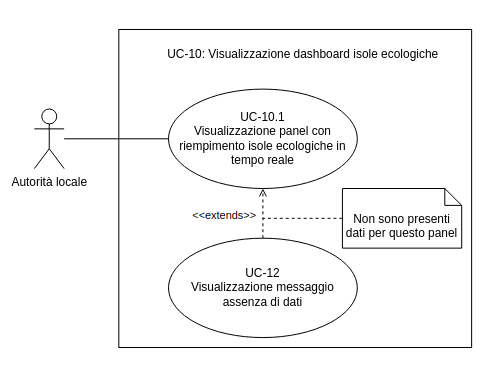
\includegraphics[width=0.75\textwidth]{analisi_dei_requisiti/UC-10.1.png}
	\captionof{figure}{UC-10.1, Visualizzazione grafico \href{https://7last.github.io/docs/rtb/documentazione-interna/glossario\#time-series}{time series\textsubscript{G}} livello di acqua}
\end{center}

\subsubsubsection{UC-10.2: Visualizzazione mappa sensori livello di acqua}
\begin{itemize}
	\item \textbf{Attore principale}: Autorità locale;
	\item \textbf{Precondizioni}:
	      \begin{enumerate}
		      \item L'autorità locale ha effettuato l'accesso al sistema ed esso è in funzione;
		      \item Il sistema ha caricato la \href{https://7last.github.io/docs/rtb/documentazione-interna/glossario\#dashboard}{dashboard\textsubscript{G}} relativa ai sensori del livello di acqua;
	      \end{enumerate}
	\item \textbf{Postcondizioni}: L'autorità locale visualizza una mappa interattiva popolata con dei marker rappresentanti la posizione dei sensori del livello di acqua;
	\item \textbf{Scenario principale}:
	      \begin{enumerate}
		      \item L'autorità locale accede alla piattaforma;
		      \item Il sistema carica i dati relativi ai sensori interrogando il database;
		      \item L'autorità locale seleziona la visualizzazione della \href{https://7last.github.io/docs/rtb/documentazione-interna/glossario\#dashboard}{dashboard\textsubscript{G}} relativa ai sensori del livello di acqua.
	      \end{enumerate}
	\item \href{https://7last.github.io/docs/rtb/documentazione-interna/glossario\#user-story}{\textbf{User story}\textsubscript{G}}:
	      Come autorità locale desidero poter visualizzare una mappa interattiva popolata con dei marker rappresentanti la posizione dei sensori del livello di acqua
	      e contenenti il loro identificativo. Essa mi consentirà di visualizzare la distribuzione dei sensori del livello di acqua nel territorio ed eventualmente interventire nel caso in cui siano presenti zone non coperte.
\end{itemize}
\begin{center}
	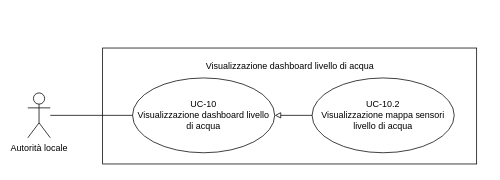
\includegraphics[width=0.75\textwidth]{analisi_dei_requisiti/UC-10.2.png}
	\captionof{figure}{UC-10.2: Visualizzazione mappa interattiva sensori livello di acqua}
\end{center}

\subsubsubsection{UC-10.3: Visualizzazione panel livello di acqua medio in un determinato periodo di tempo}
\begin{itemize}
	\item \textbf{Attore principale}: Autorità locale;
	\item \textbf{Precondizioni}:
	      \begin{enumerate}
		      \item L'autorità locale ha effettuato l'accesso al sistema ed esso è in funzione;
		      \item Il sistema ha caricato la \href{https://7last.github.io/docs/rtb/documentazione-interna/glossario\#dashboard}{dashboard\textsubscript{G}} relativa ai sensori di livello di acqua;
	      \end{enumerate}
	\item \textbf{Postcondizioni}: L'autorità locale visualizza un \textit{panel} contenente del livello di acqua medio in un determinato periodo di tempo;
	\item \textbf{Scenario principale}:
	      \begin{enumerate}
		      \item L'autorità locale accede alla piattaforma;
		      \item Il sistema carica i dati relativi ai sensori interrogando il database;
		      \item L'autorità locale seleziona la visualizzazione della \href{https://7last.github.io/docs/rtb/documentazione-interna/glossario\#dashboard}{dashboard\textsubscript{G}} relativa ai sensori di livello di acqua.
	      \end{enumerate}
	\item \href{https://7last.github.io/docs/rtb/documentazione-interna/glossario\#user-story}{\textbf{User story}\textsubscript{G}}:
	      Come autorità locale desidero poter visualizzare del livello di acqua medio in un determinato periodo di tempo
	      in modo da poterne monitorare l'andamento.
\end{itemize}
\begin{center}
	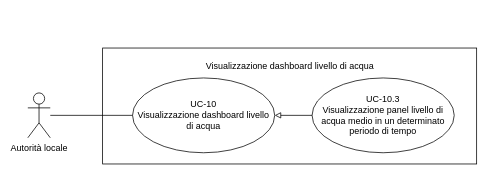
\includegraphics[width=0.75\textwidth]{analisi_dei_requisiti/UC-10.3.png}
	\captionof{figure}{UC-10.3: Visualizzazione \textit{panel} livello di acqua medio in un determinato periodo di tempo}
\end{center}

\subsubsubsection{UC-10.4: Visualizzazione panel livello di acqua in tempo reale}
\begin{itemize}
	\item \textbf{Attore principale}: Autorità locale;
	\item \textbf{Precondizioni}:
	      \begin{enumerate}
		      \item L'autorità locale ha effettuato l'accesso al sistema ed esso è in funzione;
		      \item Il sistema ha caricato la \href{https://7last.github.io/docs/rtb/documentazione-interna/glossario\#dashboard}{dashboard\textsubscript{G}} relativa ai sensori di livello di acqua;
	      \end{enumerate}
	\item \textbf{Postcondizioni}: L'autorità locale visualizza un \textit{panel} contenente il livello di acqua in tempo reale;
	\item \textbf{Scenario principale}:
	      \begin{enumerate}
		      \item L'autorità locale accede alla piattaforma;
		      \item Il sistema carica i dati relativi ai sensori interrogando il database;
		      \item L'autorità locale seleziona la visualizzazione della \href{https://7last.github.io/docs/rtb/documentazione-interna/glossario\#dashboard}{dashboard\textsubscript{G}} relativa ai sensori di livello di acqua.
	      \end{enumerate}
	\item \href{https://7last.github.io/docs/rtb/documentazione-interna/glossario\#user-story}{\textbf{User story}\textsubscript{G}}:
	      Come autorità locale desidero poter visualizzare il livello di acqua in tempo reale in modo da poterne monitorare l'andamento
	      e poterlo facilmente confrontare con i dati storici.
\end{itemize}
\begin{center}
	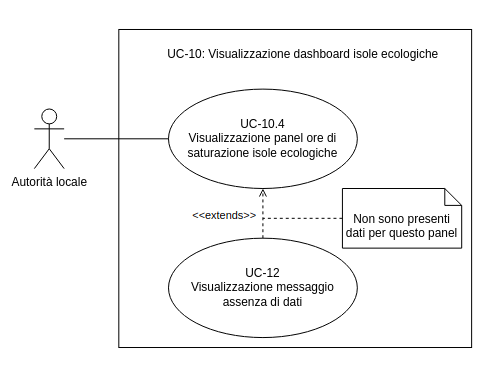
\includegraphics[width=0.75\textwidth]{analisi_dei_requisiti/UC-10.4.png}
	\captionof{figure}{UC-10.4: Visualizzazione \textit{panel} livello di acqua in tempo reale}
\end{center}

\subsubsection{UC-11: Visualizzazione messaggio assenza di dati}
\begin{itemize}
	\item \textbf{Attore principale}: Autorità locale;
	\item \textbf{Precondizioni}:
	      \begin{enumerate}
		      \item L'autorità locale accede alla piattaforma;
		      \item Il sistema carica i dati relativi ai sensori interrogando il database;
	      \end{enumerate}
	\item \textbf{Postcondizioni}: L'autorità locale visualizza un messaggio che notifica l'assenza di dati;
	\item \textbf{Scenario principale}:
	      \begin{enumerate}
		      \item L'autorità locale accede alla piattaforma;
		      \item Il sistema carica i dati relativi ai sensori interrogando il database;
		      \item Il sistema non trova dati relativi ai sensori;
		      \item Il sistema mostra un messaggio che notifica l'assenza di dati.
	      \end{enumerate}
\end{itemize}

\subsubsection{UC-12: Trasmissione dati temperatura}
\begin{itemize}
	\item \textbf{Attore principale}: \href{https://7last.github.io/docs/rtb/documentazione-interna/glossario\#sensore}{Sensore\textsubscript{G}};
	\item \textbf{Precondizioni}: Il \href{https://7last.github.io/docs/rtb/documentazione-interna/glossario\#sensore}{sensore\textsubscript{G}} è attivo e collegato al sistema;
	\item \textbf{Postcondizioni}: I dati inviati dal \href{https://7last.github.io/docs/rtb/documentazione-interna/glossario\#sensore}{sensore\textsubscript{G}} sono stati elaborati e memorizzati nel sistema;
	\item \textbf{Scenario principale}:
	      \begin{enumerate}
		      \item Il \href{https://7last.github.io/docs/rtb/documentazione-interna/glossario\#sensore}{sensore\textsubscript{G}} effettua una misurazione di temperatura;
		      \item Il \href{https://7last.github.io/docs/rtb/documentazione-interna/glossario\#sensore}{sensore\textsubscript{G}} formatta i dati da inviare al sistema, includendo oltre alle misurazioni l'identificativo del \href{https://7last.github.io/docs/rtb/documentazione-interna/glossario\#sensore}{sensore\textsubscript{G}},
		            il timestamp, e la sua posizione geografica;
		      \item Il \href{https://7last.github.io/docs/rtb/documentazione-interna/glossario\#sensore}{sensore\textsubscript{G}} invia i dati al sistema.
	      \end{enumerate}
	\item \href{https://7last.github.io/docs/rtb/documentazione-interna/glossario\#user-story}{\textbf{User story}\textsubscript{G}}: Come \href{https://7last.github.io/docs/rtb/documentazione-interna/glossario\#sensore}{sensore\textsubscript{G}}, desidero poter inviare al sistema le rilevazioni della temperatura.
\end{itemize}

\begin{center}
	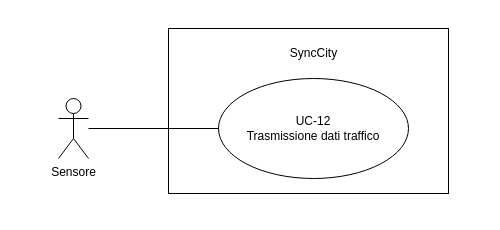
\includegraphics[width=0.6\textwidth]{analisi_dei_requisiti/UC-12.png}
	\captionof{figure}{UC-12: Trasmissione dati temperatura}
\end{center}

\subsubsection{UC-13: Trasmissione dati umidità}
\begin{itemize}
	\item \textbf{Attore principale}: \href{https://7last.github.io/docs/rtb/documentazione-interna/glossario\#sensore}{Sensore\textsubscript{G}};
	\item \textbf{Precondizioni}: Il \href{https://7last.github.io/docs/rtb/documentazione-interna/glossario\#sensore}{sensore\textsubscript{G}} è attivo e collegato al sistema;
	\item \textbf{Postcondizioni}: I dati inviati dal \href{https://7last.github.io/docs/rtb/documentazione-interna/glossario\#sensore}{sensore\textsubscript{G}} sono stati elaborati e memorizzati nel sistema;
	\item \textbf{Scenario principale}:
	      \begin{enumerate}
		      \item Il \href{https://7last.github.io/docs/rtb/documentazione-interna/glossario\#sensore}{sensore\textsubscript{G}} effettua una misurazione dell'umidità;
		      \item Il \href{https://7last.github.io/docs/rtb/documentazione-interna/glossario\#sensore}{sensore\textsubscript{G}} formatta i dati da inviare al sistema, includendo oltre alle misurazioni l'identificativo del \href{https://7last.github.io/docs/rtb/documentazione-interna/glossario\#sensore}{sensore\textsubscript{G}},
		            il timestamp, e la sua posizione geografica;
		      \item Il \href{https://7last.github.io/docs/rtb/documentazione-interna/glossario\#sensore}{sensore\textsubscript{G}} invia i dati al sistema.
	      \end{enumerate}
	\item \href{https://7last.github.io/docs/rtb/documentazione-interna/glossario\#user-story}{\textbf{User story}\textsubscript{G}}: Come \href{https://7last.github.io/docs/rtb/documentazione-interna/glossario\#sensore}{sensore\textsubscript{G}}, desidero poter inviare al sistema le rilevazioni dell'umidità.
\end{itemize}

\begin{center}
	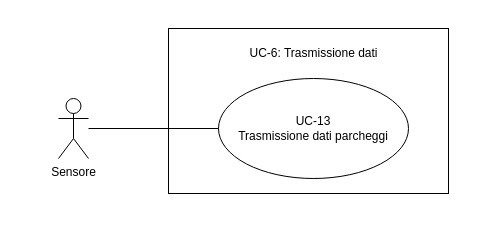
\includegraphics[width=0.6\textwidth]{analisi_dei_requisiti/UC-13.png}
	\captionof{figure}{UC-13: Trasmissione dati umidità}
\end{center}

\subsubsection{UC-14: Trasmissione dati qualità dell'aria}
\begin{itemize}
	\item \textbf{Attore principale}: \href{https://7last.github.io/docs/rtb/documentazione-interna/glossario\#sensore}{Sensore\textsubscript{G}};
	\item \textbf{Precondizioni}: Il \href{https://7last.github.io/docs/rtb/documentazione-interna/glossario\#sensore}{sensore\textsubscript{G}} è attivo e collegato al sistema;
	\item \textbf{Postcondizioni}: I dati inviati dal \href{https://7last.github.io/docs/rtb/documentazione-interna/glossario\#sensore}{sensore\textsubscript{G}} sono stati elaborati e memorizzati nel sistema;
	\item \textbf{Scenario principale}:
	      \begin{enumerate}
		      \item Il \href{https://7last.github.io/docs/rtb/documentazione-interna/glossario\#sensore}{sensore\textsubscript{G}} effettua una misurazione della quantità di precipitazioni;
		      \item Il \href{https://7last.github.io/docs/rtb/documentazione-interna/glossario\#sensore}{sensore\textsubscript{G}} formatta i dati da inviare al sistema, includendo oltre alle misurazioni l'identificativo del \href{https://7last.github.io/docs/rtb/documentazione-interna/glossario\#sensore}{sensore\textsubscript{G}},
		            il timestamp, e la sua posizione geografica;
		      \item Il \href{https://7last.github.io/docs/rtb/documentazione-interna/glossario\#sensore}{sensore\textsubscript{G}} invia i dati al sistema.
	      \end{enumerate}
	\item \href{https://7last.github.io/docs/rtb/documentazione-interna/glossario\#user-story}{\textbf{User story}\textsubscript{G}}:
	      Come \href{https://7last.github.io/docs/rtb/documentazione-interna/glossario\#sensore}{sensore\textsubscript{G}}, desidero poter inviare al sistema le rilevazioni della qualità dell'aria.
\end{itemize}

\begin{center}
	\includegraphics[width=0.6\textwidth]{analisi_dei_requisiti/UC-14.png}
	\captionof{figure}{UC-14: Trasmissione dati precipitazioni}
\end{center}

\subsubsection{UC-15: Trasmissione dati precipitazioni}
\begin{itemize}
	\item \textbf{Attore principale}: \href{https://7last.github.io/docs/rtb/documentazione-interna/glossario\#sensore}{Sensore\textsubscript{G}};
	\item \textbf{Precondizioni}: Il \href{https://7last.github.io/docs/rtb/documentazione-interna/glossario\#sensore}{sensore\textsubscript{G}} è attivo e collegato al sistema;
	\item \textbf{Postcondizioni}: I dati inviati dal \href{https://7last.github.io/docs/rtb/documentazione-interna/glossario\#sensore}{sensore\textsubscript{G}} sono stati elaborati e memorizzati nel sistema;
	\item \textbf{Scenario principale}:
	      \begin{enumerate}
		      \item Il \href{https://7last.github.io/docs/rtb/documentazione-interna/glossario\#sensore}{sensore\textsubscript{G}} effettua una misurazione della quantità di precipitazioni;
		      \item Il \href{https://7last.github.io/docs/rtb/documentazione-interna/glossario\#sensore}{sensore\textsubscript{G}} formatta i dati da inviare al sistema, includendo oltre alle misurazioni l'identificativo del \href{https://7last.github.io/docs/rtb/documentazione-interna/glossario\#sensore}{sensore\textsubscript{G}},
		            il timestamp, e la sua posizione geografica;
		      \item Il \href{https://7last.github.io/docs/rtb/documentazione-interna/glossario\#sensore}{sensore\textsubscript{G}} invia i dati al sistema.
	      \end{enumerate}
	\item \href{https://7last.github.io/docs/rtb/documentazione-interna/glossario\#user-story}{\textbf{User story}\textsubscript{G}}: Come \href{https://7last.github.io/docs/rtb/documentazione-interna/glossario\#sensore}{sensore\textsubscript{G}}, desidero poter inviare al sistema le rilevazioni della quantità di precipitazioni.
\end{itemize}

\begin{center}
	\includegraphics[width=0.6\textwidth]{analisi_dei_requisiti/UC-15.png}
	\captionof{figure}{UC-15: Trasmissione dati precipitazioni}
\end{center}

\subsubsection{UC-16: Trasmissione dati traffico}
\begin{itemize}
	\item \textbf{Attore principale}: \href{https://7last.github.io/docs/rtb/documentazione-interna/glossario\#sensore}{Sensore\textsubscript{G}};
	\item \textbf{Precondizioni}: Il \href{https://7last.github.io/docs/rtb/documentazione-interna/glossario\#sensore}{sensore\textsubscript{G}} è attivo e collegato al sistema;
	\item \textbf{Postcondizioni}: I dati inviati dal \href{https://7last.github.io/docs/rtb/documentazione-interna/glossario\#sensore}{sensore\textsubscript{G}} sono stati elaborati e memorizzati nel sistema;
	\item \textbf{Scenario principale}:
	      \begin{enumerate}
		      \item Il \href{https://7last.github.io/docs/rtb/documentazione-interna/glossario\#sensore}{sensore\textsubscript{G}} effettua una misurazione del traffico;
		      \item Il \href{https://7last.github.io/docs/rtb/documentazione-interna/glossario\#sensore}{sensore\textsubscript{G}} formatta i dati da inviare al sistema, includendo oltre alle misurazioni l'identificativo del \href{https://7last.github.io/docs/rtb/documentazione-interna/glossario\#sensore}{sensore\textsubscript{G}},
		            il timestamp, e la sua posizione geografica;
		      \item Il \href{https://7last.github.io/docs/rtb/documentazione-interna/glossario\#sensore}{sensore\textsubscript{G}} invia i dati al sistema.
	      \end{enumerate}
	\item \href{https://7last.github.io/docs/rtb/documentazione-interna/glossario\#user-story}{\textbf{User story}\textsubscript{G}}: Come \href{https://7last.github.io/docs/rtb/documentazione-interna/glossario\#sensore}{sensore\textsubscript{G}}, desidero poter inviare al sistema le rilevazioni sui dati del traffico.
\end{itemize}

\begin{center}
	\includegraphics[width=0.6\textwidth]{analisi_dei_requisiti/UC-16.png}
	\captionof{figure}{UC-16: Trasmissione dati traffico}
\end{center}


\subsubsection{UC-17: Trasmissione dati colonnine di ricarica}
\begin{itemize}
	\item \textbf{Attore principale}: \href{https://7last.github.io/docs/rtb/documentazione-interna/glossario\#sensore}{Sensore\textsubscript{G}};
	\item \textbf{Precondizioni}: Il \href{https://7last.github.io/docs/rtb/documentazione-interna/glossario\#sensore}{sensore\textsubscript{G}} è attivo e collegato al sistema;
	\item \textbf{Postcondizioni}: I dati inviati dal \href{https://7last.github.io/docs/rtb/documentazione-interna/glossario\#sensore}{sensore\textsubscript{G}} sono stati elaborati e memorizzati nel sistema;
	\item \textbf{Scenario principale}:
	      \begin{enumerate}
		      \item Il \href{https://7last.github.io/docs/rtb/documentazione-interna/glossario\#sensore}{sensore\textsubscript{G}} effettua una misurazione dello stato e l'occupazione delle colonnine di ricarica;
		      \item Il \href{https://7last.github.io/docs/rtb/documentazione-interna/glossario\#sensore}{sensore\textsubscript{G}} formatta i dati da inviare al sistema, includendo oltre alle misurazioni l'identificativo del \href{https://7last.github.io/docs/rtb/documentazione-interna/glossario\#sensore}{sensore\textsubscript{G}},
		            il timestamp, e la sua posizione geografica;
		      \item Il \href{https://7last.github.io/docs/rtb/documentazione-interna/glossario\#sensore}{sensore\textsubscript{G}} invia i dati al sistema.
	      \end{enumerate}
	\item \href{https://7last.github.io/docs/rtb/documentazione-interna/glossario\#user-story}{\textbf{User story}\textsubscript{G}}: Come \href{https://7last.github.io/docs/rtb/documentazione-interna/glossario\#sensore}{sensore\textsubscript{G}}, desidero poter inviare al sistema le rilevazioni sullo stato e l'occupazione delle colonnine di ricarica.
\end{itemize}
\begin{center}
	\includegraphics[width=0.6\textwidth]{analisi_dei_requisiti/UC-17.png}
	\captionof{figure}{UC-17: Trasmissione dati colonnine di ricarica}
\end{center}

\subsubsection{UC-18: Trasmissione dati parcheggi}
\begin{itemize}
	\item \textbf{Attore principale}: \href{https://7last.github.io/docs/rtb/documentazione-interna/glossario\#sensore}{Sensore\textsubscript{G}};
	\item \textbf{Precondizioni}: Il \href{https://7last.github.io/docs/rtb/documentazione-interna/glossario\#sensore}{sensore\textsubscript{G}} è attivo e collegato al sistema;
	\item \textbf{Postcondizioni}: I dati inviati dal \href{https://7last.github.io/docs/rtb/documentazione-interna/glossario\#sensore}{sensore\textsubscript{G}} sono stati elaborati e memorizzati nel sistema;
	\item \textbf{Scenario principale}:
	      \begin{enumerate}
		      \item Il \href{https://7last.github.io/docs/rtb/documentazione-interna/glossario\#sensore}{sensore\textsubscript{G}} effettua una misurazione dello stato di riempimento del parcheggio;
		      \item Il \href{https://7last.github.io/docs/rtb/documentazione-interna/glossario\#sensore}{sensore\textsubscript{G}} formatta i dati da inviare al sistema, includendo oltre alle misurazioni l'identificativo del \href{https://7last.github.io/docs/rtb/documentazione-interna/glossario\#sensore}{sensore\textsubscript{G}},
		            il timestamp, e la sua posizione geografica;
		      \item Il \href{https://7last.github.io/docs/rtb/documentazione-interna/glossario\#sensore}{sensore\textsubscript{G}} invia i dati al sistema.
	      \end{enumerate}
	\item \href{https://7last.github.io/docs/rtb/documentazione-interna/glossario\#user-story}{\textbf{User story}\textsubscript{G}}: Come \href{https://7last.github.io/docs/rtb/documentazione-interna/glossario\#sensore}{sensore\textsubscript{G}}, desidero poter inviare al sistema le rilevazioni sull'occupazione dei parcheggi.
\end{itemize}

\begin{center}
	\includegraphics[width=0.6\textwidth]{analisi_dei_requisiti/UC-18.png}
	\captionof{figure}{UC-18: Trasmissione dati parcheggi}
\end{center}

\subsubsection{UC-19: Trasmissione dati isole ecologiche}
\begin{itemize}
	\item \textbf{Attore principale}: \href{https://7last.github.io/docs/rtb/documentazione-interna/glossario\#sensore}{Sensore\textsubscript{G}};
	\item \textbf{Precondizioni}: Il \href{https://7last.github.io/docs/rtb/documentazione-interna/glossario\#sensore}{sensore\textsubscript{G}} è attivo e collegato al sistema;
	\item \textbf{Postcondizioni}: I dati inviati dal \href{https://7last.github.io/docs/rtb/documentazione-interna/glossario\#sensore}{sensore\textsubscript{G}} sono stati elaborati e memorizzati nel sistema;
	\item \textbf{Scenario principale}:
	      \begin{enumerate}
		      \item Il \href{https://7last.github.io/docs/rtb/documentazione-interna/glossario\#sensore}{sensore\textsubscript{G}} effettua una misurazione dello stato di riempimento delle isole ecologiche;
		      \item Il \href{https://7last.github.io/docs/rtb/documentazione-interna/glossario\#sensore}{sensore\textsubscript{G}} formatta i dati da inviare al sistema, includendo oltre alle misurazioni l'identificativo del \href{https://7last.github.io/docs/rtb/documentazione-interna/glossario\#sensore}{sensore\textsubscript{G}},
		            il timestamp, e la sua posizione geografica;
		      \item Il \href{https://7last.github.io/docs/rtb/documentazione-interna/glossario\#sensore}{sensore\textsubscript{G}} invia i dati al sistema.
	      \end{enumerate}
	\item \href{https://7last.github.io/docs/rtb/documentazione-interna/glossario\#user-story}{\textbf{User story}\textsubscript{G}}: Come \href{https://7last.github.io/docs/rtb/documentazione-interna/glossario\#sensore}{sensore\textsubscript{G}}, desidero poter inviare al sistema le rilevazioni sullo stato di riempimento delle isole ecologiche.
\end{itemize}

\begin{center}
	\includegraphics[width=0.6\textwidth]{analisi_dei_requisiti/UC-19.png}
	\captionof{figure}{UC-19: Trasmissione dati isole ecologiche}
\end{center}

\subsubsection{UC-20: Trasmissione dati livello di acqua}
\begin{itemize}
	\item \textbf{Attore principale}: \href{https://7last.github.io/docs/rtb/documentazione-interna/glossario\#sensore}{Sensore\textsubscript{G}};
	\item \textbf{Precondizioni}: Il \href{https://7last.github.io/docs/rtb/documentazione-interna/glossario\#sensore}{sensore\textsubscript{G}} è attivo e collegato al sistema;
	\item \textbf{Postcondizioni}: I dati inviati dal \href{https://7last.github.io/docs/rtb/documentazione-interna/glossario\#sensore}{sensore\textsubscript{G}} sono stati elaborati e memorizzati nel sistema;
	\item \textbf{Scenario principale}:
	      \begin{enumerate}
		      \item Il \href{https://7last.github.io/docs/rtb/documentazione-interna/glossario\#sensore}{sensore\textsubscript{G}} effettua una misurazione del livello di acqua;
		      \item Il \href{https://7last.github.io/docs/rtb/documentazione-interna/glossario\#sensore}{sensore\textsubscript{G}} formatta i dati da inviare al sistema, includendo oltre alle misurazioni l'identificativo del \href{https://7last.github.io/docs/rtb/documentazione-interna/glossario\#sensore}{sensore\textsubscript{G}},
		            il timestamp, e la sua posizione geografica;
		      \item Il \href{https://7last.github.io/docs/rtb/documentazione-interna/glossario\#sensore}{sensore\textsubscript{G}} invia i dati al sistema.
	      \end{enumerate}
	\item \href{https://7last.github.io/docs/rtb/documentazione-interna/glossario\#user-story}{\textbf{User story}\textsubscript{G}}: Come \href{https://7last.github.io/docs/rtb/documentazione-interna/glossario\#sensore}{sensore\textsubscript{G}}, desidero poter inviare al sistema le rilevazioni sul livello di acqua.
\end{itemize}

\begin{center}
	\includegraphics[width=0.6\textwidth]{analisi_dei_requisiti/UC-20.png}
	\captionof{figure}{UC-20: Trasmissione dati livello di acqua}
\end{center}

\subsubsection{UC-21: Applicazione filtro sensore}
\begin{itemize}
	\item \textbf{Attore principale}: Autorità locale;
	\item \textbf{Precondizioni}:
	      \begin{enumerate}
		      \item L'autorità locale ha effettuato l'accesso al sistema ed esso è in funzione;
		      \item Il sistema ha caricato i dati interrogando il database;
		      \item L'autorità locale visualizza una \href{https://7last.github.io/docs/rtb/documentazione-interna/glossario\#dashboard}{dashboard\textsubscript{G}}.
	      \end{enumerate}
	\item \textbf{Postcondizioni}: L'autorità locale applica un filtro ai dati visualizzati in modo da poter visualizzare solo i dati relativi ad un \href{https://7last.github.io/docs/rtb/documentazione-interna/glossario\#sensore}{sensore\textsubscript{G}} specifico;
	\item \textbf{Scenario principale}:
	      \begin{enumerate}
		      \item L'autorità locale visualizza una \href{https://7last.github.io/docs/rtb/documentazione-interna/glossario\#dashboard}{dashboard\textsubscript{G}};
		      \item L'autorità locale seleziona il \href{https://7last.github.io/docs/rtb/documentazione-interna/glossario\#sensore}{sensore\textsubscript{G}} di cui vuole visualizzare i dati;
	      \end{enumerate}
	\item \href{https://7last.github.io/docs/rtb/documentazione-interna/glossario\#user-story}{\textbf{User story}\textsubscript{G}}:
	      Come autorità locale desidero poter visualizzare solo i dati relativi ad un \href{https://7last.github.io/docs/rtb/documentazione-interna/glossario\#sensore}{sensore\textsubscript{G}} specifico in modo da poter facilmente
	      monitorare i dati di un \href{https://7last.github.io/docs/rtb/documentazione-interna/glossario\#sensore}{sensore\textsubscript{G}} specifico e circoscrivere l'analisi ai dati di interesse.
\end{itemize}
\begin{center}
	\includegraphics[width=0.6\textwidth]{analisi_dei_requisiti/UC-21.png}
	\captionof{figure}{UC-21: Applicazione filtro \href{https://7last.github.io/docs/rtb/documentazione-interna/glossario\#sensore}{sensore\textsubscript{G}}}
\end{center}
